%!TEX root = ../thesis.tex

\chapter{Implementierung und Proof of Concept} % (fold)
\label{cha:implementierung_und_evaluation}

Dieses Kapitel beinhaltet Informationen über die Implementierung von Connectoren für die im Abschnitt \ref{sec:lernplattformen_und_soziale_online_netzwerke} vorgestellten Plattformen. Diese wurden nicht nur ausgewählt, weil sie fast alle weit verbreitet sind, sondern weil sie auch verschiedenen Klassen von Plattformen angehören. Moodle und Canvas gehören zu der Klasse der Lernplattformen und beinhalten eine klassische Forenstruktur für Diskussionen. Die Plattformen Facebook und Google+ sind soziale Online-Netzwerke, die zurzeit einen großen Aufschwung erleben. Und zuletzt noch Youtube, das als Videoportal anderen das bereitstellen von Videomaterial und das Diskutieren über diese ermöglicht. Während alle fünf Plattformen auf REST (Moodle auch SOAP) als Architektur ihrer APIs setzten, sind die Formen für die Authentifizierung teils sehr unterschiedlich, auch wenn sie den selben Mechanismus einsetzten.

In den folgenden Abschnitten wird erklärt wie man auf die Daten der einzelnen Plattformen über ihre APIs zugreifen kann und welche Voraussetzungen dafür erfüllt sein müssen. Gleichfalls wird beschreiben, wie der Zugriff auf diese API innerhalb der Programmiersprache Java funktionieren kann, da diese APIs in der Regel für Webanwendungen ausgelegt sind. Danach wird noch gezeigt welches Mapping zwischen den Ressourcen der Plattformen und dem SIOC-Format gewählt wurde. Traten bei der Implementierung Besonderheiten auf, die für andere Entwickler interessant sein könnten, wurden diese in einen eigenen Abschnitt des betreffenden Connectors aufgeführt.

Der Schluss des Kapitels bildet ein \enquote{Proof of Concept} (Englisch für Machbarkeitsnachweis), der demonstrieren soll wie ein Programm zu Synchronisation von Beiträgen mit SOCC aussehen kann und wie es funktioniert.

\section{Verwendete Programme und Bibliotheken} % (fold)
\label{sec:verwendete_bibliotheken_und_programme}

An diesen Punkt soll noch kurz auf zusätzliche Programm und Bibliotheken eingegangen werden, die für die Entwicklung der einzelnen Connectoren hilfreich waren. 

\begin{description}
    \item[\textbf{Apache Maven:}] Für die Entwicklung der Programme und Bibliotheken dieser Arbeit wurde das Build-Management Programm \texttt{Maven}\footnote{http://maven.apache.org/} von Apache eingesetzt. Mit diesem ist es auf einfache Art möglich Java-Programme zu Verwalten und zu Erstellen. So ist nur mit einer einzigen XML-Datei (\texttt{pom.xml}) möglich die Abhängigkeiten festzulegen, das Programm zu kompilieren, zu testen und es auszuliefern. Maven schreibt eine feste Ordnerstruktur für ein Projekt vor wie der Produktivquellcode, dafür nötige Ressource (Bilder, Texte,\dots) und der Quellcode zum Testen geordnet werden sollen. Die Abhängigkeiten werden automatisch aus zentralen Repositorien heruntergeladen und in das Projekt eingebunden. So muss dies nicht umständlich von Hand geschehen und spart so Arbeit.

    \item[\textbf{RDF2Go:}] Für die Programmiersprache Java gibt es einige Bibliotheken mit denen RDF-Daten verarbeitet werden können. Wie zum Beispiel \emph{Sesame}\footnote{\url{http://www.openrdf.org}}, \emph{Apache Jena}\footnote{\url{http://jena.apache.org}} oder \emph{JRDF}\footnote{\url{http://jrdf.sourceforge.net/}}. Jede dieser Bibliotheken bietet einen Triplestore und eine API für das Arbeiten mit RDF-Triples. Stellt sich nur die Frage welche man von ihnen auszuwählen soll? 

    Einen Ausweg aus dieser Misere bietet \emph{RDF2Go}\footnote{\url{http://semanticweb.org/wiki/RDF2Go}}. RDF2Go abstrahiert andere Triplestores über eine einheitliche API und erlaubt es den Triplestore später wechseln zu können. Dazu muss für den Triplestore nur ein Adapter für RDF2Go implementiert werden, welche aktuell für Sesame und Apache Jena vorhanden sind. Für RDF2Go existiert auch ein Programm RDFReactor mit dem aus Ontologien in RDFS und OWL Java-Klassen generieren werden können. So muss nicht jedes Objekt mühevoll Triple für Triple zusammengebaut werden. 

    \item[\textbf{Handy-URI-Templates:}] Bei der Arbeit mit RDF kommt man zwangsläufig um das Verarbeiten von URIs nicht herum. Um diese Arbeit zu erleichtern, wird bei der Implementierung die Java-Bibliothek \emph{Handy-URI-Templates}\footnote{\url{https://github.com/damnhandy/Handy-URI-Templates}} eingesetzt. Diese implementiert den \emph{RFC6570}\footnote{\url{http://tools.ietf.org/html/rfc6570}}, welches eine Sprache für URI-Vorlagen definiert. Zum Erzeugen einer URI muss nur eine solche Vorlage definiert und mit der API von Handy-URI-Templates mit Werten gefüllt werden. Die Vorlage \texttt{http://www.example.org\{?x,y\}} würde so mit den Werten \texttt{x=42} und \texttt{y=23} die URI \texttt{http://www.example.org?x=42\&y=23} entstehen lassen.
\end{description}

% section verwendete_bibliotheken_und_programme (end)

\section{Implementierung der Connectoren} % (fold)
\label{sec:implementierung_der_connectoren}

In diesen Abschnitt soll nun beschrieben werden, wie Connectoren für die in Abschnitt \ref{sec:lernplattformen_und_soziale_online_netzwerke} vorgestellten Plattformen implementiert werden können. Dafür wird darauf eingegangen mit welcher Art von API auf die Ressourcen der einzelnen Plattformen zugegriffen werden und wie man deren Datenstruktur in SIOC abbilden kann. Ebenfalls werden auftretende Probleme und wenn möglich deren Lösung gezeigt.

\subsection{Allgemeine Informationen zum Mapping nach SIOC} % (fold)
\label{sub:allgemeine_informationen_zum_mapping_nach_sioc}

Innerhalb der Beschreibungen des Mappings nach SIOC werden, zur besseren Übersicht und einfacheren Lesbarkeit, Platzhalt für einige URIs benutzt. Welche Platzhalten dies sind und für welche URI sie stehen ist aus Tabelle \ref{tbl:platzhalter_fuer_sioc_mapping} zu entnehmen.

Da einige Eigenschaften der Klassen von SIOC bei allen Plattformen mit ähnlichen Werten belegt werden und sich nur vom Aufruf der API unterscheiden, sollen zuvor für die SIOC-Klassen \texttt{sioc:UserAccount}, \texttt{sioc:Forum}, \texttt{sioc:Thread} und \texttt{sioc:Post} die Eigenschaften beschrieben werden, die überall verwendet werden.

\begin{description}
    \item[\textbf{\texttt{sioc:UserAccount}:}]  Für die Klasse \texttt{sioc:UserAccount} ist die Angabe von vier Eigenschaften wichtig. Die erste ist \texttt{sioc:Id} mit der die ID des Benutzerkontos angegeben wird und \texttt{sioc:name} für den den Benutzernamen. Aus Kompatibilitätsgründen mit FOAF und für den ClientManager wird die ID des Benutzers noch mit \texttt{foaf:accountName} angegeben und die URI zum verwendeten Service mit \texttt{foaf:accountServiceHomepage}. Die Angabe der Daten zur Authentifizierung erfolgt mit der Eigenschaft \texttt{siocsa:accountAuthentication}.

    \item[\textbf{\texttt{sioc:Forum}:}] Jedes Forum hat seine eigene ID, die wie bei \texttt{sioc:UserAccount} unter der Eigenschaft \texttt{sioc:id} abgelegt wird. Ebenfalls bekommt jedes Forum einen Namen mit \texttt{sioc:name}. Jedes Forum hat eine \texttt{sioc:Site} von der es gehostet wird (\texttt{sioc:has\_host}). Ein Forum kann als Container für Beiträge deinen, die mit der Eigenschaft \texttt{sioc:container\_of} mit dem Forum verbunden werden. Zugleich kann es auch Threads mit \texttt{sioc:parent\_of} enthalten. 

    \item[\textbf{\texttt{sioc:Thread}:}] Ein Thread enthält ebenfalls wieder eine ID und einen Namen und enthält nur Beiträge der Klasse \texttt{sioc:Post} mit \texttt{sioc:container\_of} und ist immer ein Teil eines bestimmten Forums mit \texttt{sioc:has\_parent}.

    \item[\textbf{\texttt{sioc:Post}:}] Jeder Beitrag hat eine, für die Seite der Plattform eindeutige ID mit \texttt{sioc:id}. Mit der Eigenschaft \texttt{sioc:creator} wird der \texttt{sioc:UserAccount} des Autors festgelegt und mit \texttt{sioc:content} der Inhalt des Beitrags. Besitzt ein Beitrag eine Titel, wird dieser mit \texttt{sioc:title} gespeichert. Der Zeitpunkt der Erstellung kommt nach \texttt{dcterms:created} und der bei einer Modifikation nach \texttt{dcterms:modified}. Beiträge gehören immer zu einen Forum oder Thread welches mit \texttt{sioc:has\_container} angegeben wird. Auch können Beiträge Kommentare mit \texttt{sioc:has\_reply} enthalten oder selber Kommentare auf andere Beiträge mit \texttt{sioc:reply\_of} sein.
\end{description}

\begin{table}[ht]
    \centering
    \caption{Allgemeine Platzhalter und deren Beschreibung für das Mapping nach SIOC}
    \begin{tabular}{l|p{11cm}}
        \textbf{Platzhalter} & \textbf{Bedeutung} \\ 
        \hline
        \texttt{\{rootUri\}} & Die Basis-URI einer Webseite (Schema + Authority\footnotemark). Für Facebook wäre dies zum Beispiel \texttt{https://www.facebook.com} \\
        \texttt{\{siteUri\}} & URI für eine \texttt{sioc:Site} \\
        \texttt{\{serviceUri\}} & URI für einen \texttt{sioc:Service} \\
        \texttt{\{userAccountUri\}} & URI für einen \texttt{sioc:UserAccount} \\
        \texttt{\{forumUri\}} & URI für ein \texttt{sioc:Forum} \\
        \texttt{\{threadUri\}} & URI für ein \texttt{sioc:Thread} \\
        \texttt{\{postUri\}} & URI für ein \texttt{sioc:Post}
    \end{tabular}
    \label{tbl:platzhalter_fuer_sioc_mapping}
\end{table}
\footnotetext{\url{http://tools.ietf.org/html/rfc3986\#section-3}}

% subsection allgemeine_informationen_zum_mapping_nach_sioc (end)

\subsection{Allgemeine Probleme und Lösungen bei der Implementierung} % (fold)
\label{sub:allgemeine_probleme}

Bei der Implementierung der Connectoren treten ab und zu Probleme auf, die unabhängig von der verwendeten API gelöst werden mussten. Hier sollen diese Probleme und deren Lösung vorgestellt werden. 

\subsubsection{Doppelte Beiträge beim Synchronisieren} % (fold)
\label{ssub:doppelte_beitraege_beim_synchronisieren}

Sollen zwei Container auf unterschiedlichen Plattformen synchronisiert werden, tritt automatisch das Problem auf, dass Beiträge die von A nach B geschrieben wurden beim auslesen von B wieder bei A als \enquote{neuer} Beitrag landen würde, obwohl er ursprünglich von dort kam. Dies würde ohne Eingreifen zu einer Dauerschleife führen, bei der die selben Beiträge immer hin und her geschrieben werden. 

Aus diesem Grund wird vor dem Schreiben eines Beitrags eine Art Wasserzeichen zum Inhalt hinzugefügt. Dieses Wasserzeichen besteht aus der Zeichenkette \enquote{--- forwarded by SOCC \{siteUri\} ---}. Der Platzhalter \enquote{\{siteUri\}} wird dabei durch die URI der Seite ersetzt von der der Beitrag gekommen ist. Hierzu muss jedem Beitrag mit der Eigenschaft \texttt{dcterms:isPartOf} die URI des \texttt{sioc:Site}-Objekts zu dem der Beitrag gehört hinzugefügt werden. Wird nun eine Beitrag gelesen, der ursprünglich von der Seite des Connectors kam, wird dieser ignoriert. Enthält dagegen der Beitrag schon eine Wasserzeichen mit der URI einer anderen Seite, wird kein neues Wasserzeichen hinzugefügt.

% subsubsection synchronisieren_von_beitrage (end)

\subsubsection{Rekonstruktion der Kommentarstruktur} % (fold)
\label{ssub:rekonstruktion_der_kommentarstruktur}

Bei der Synchronisation ist es ebenso wichtig die Struktur von Kommentaren beizubehalten. Wenn Beitrag A2 ein Kommentar auf Beitrag A1 in Seite A ist, dann muss diese Struktur beim Synchronisieren auf Seite B mit den Beiträgen B1 und B2 erhalten bleiben.

\begin{figure}[ht]
    \centering
    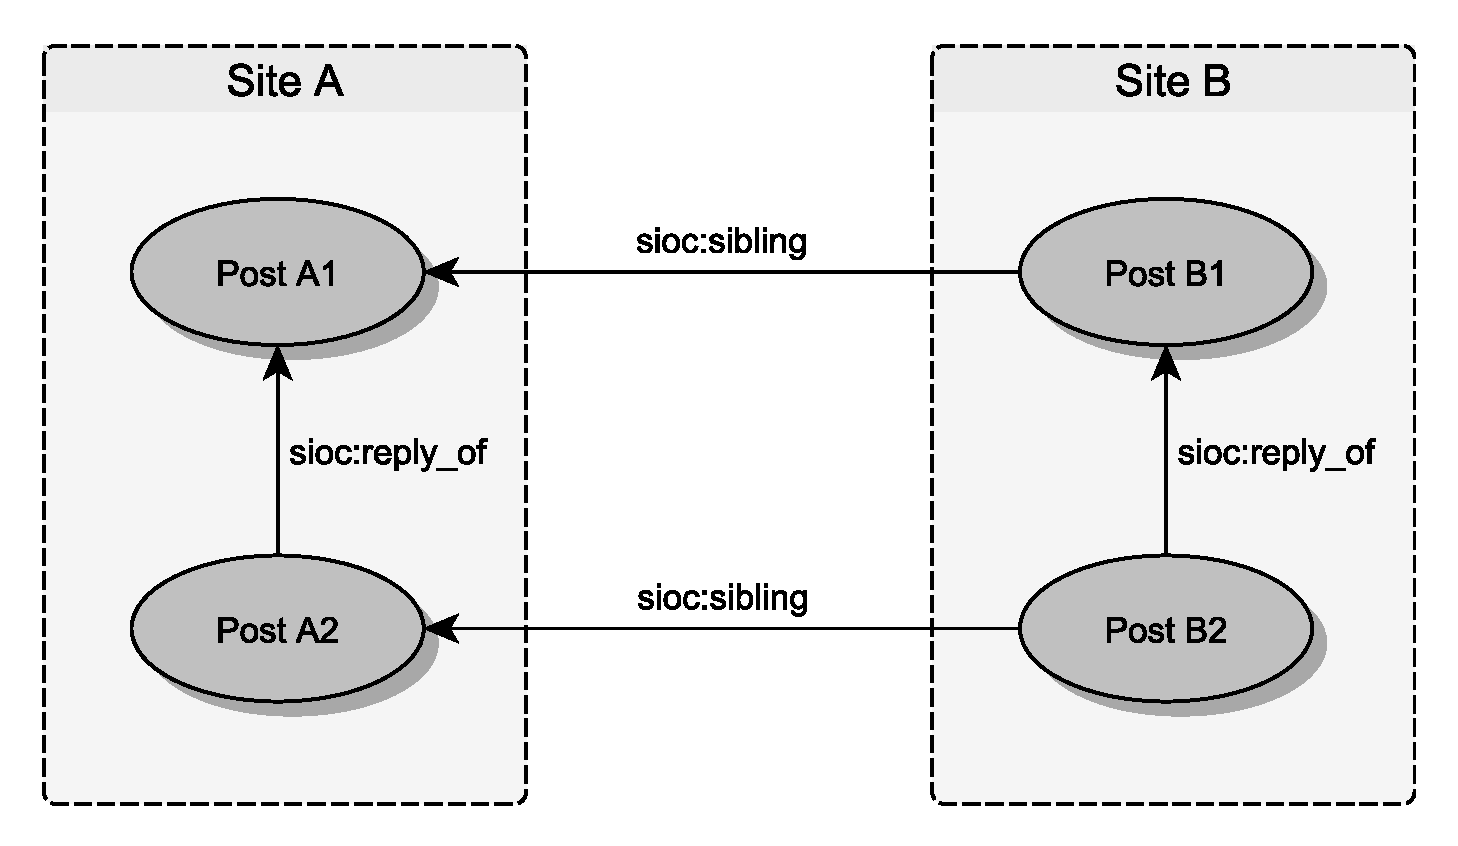
\includegraphics[
        width=0.7\textwidth,
        keepaspectratio=true
    ]{assets/images/comment_structuring}
    \caption{Erhalten der Kommentarstruktur beim Schreiben von Beiträgen}
    \label{fig:kommentarsturktur_beim_schreiben}
\end{figure}

Hierzu wird nach dem Schreiben eines Beitrags mit der Eigenschaft \texttt{sioc:sibling} (Englisch für Geschwister) die URI zum original Beitrag beim geschriebenen Beitrag festgehalten. Taucht nun beim Schreiben ein Beitrag auf, der ein Kommentar auf den mit \texttt{sioc:sibling} gespeicherten Beitrags ist, kann dieser an die richtige Stelle als Kommentar geschrieben werden. Der RDF-Graph nach dem Synchronisieren ist in Abbildung \ref{ssub:rekonstruktion_der_kommentarstruktur} zu sehen. 

Leider funktioniert diese Methode erst wenn die entsprechenden Beziehungen vorhanden sind. Werden Beiträge von Seite A zur Seite B geschrieben funktioniert dies tadellos. Wird aber nun auf Seite B ein Kommentar auf einen dieser Beiträge geschrieben und zu Seite A geschickt, kann diese den Beitrag nicht richtig einfügen, da \texttt{sioc:reply\_of} natürlich auf einen Beitrag von Seite B zeigt und die \texttt{sioc:sibling} Informationen auf Seite A fehlen.

% subsubsection rekonstruktion_der_kommentarstruktur (end)

% subsection allgemeine_probleme (end)

\subsection{MoodleConnector} % (fold)
\label{sub:moodle_connector}

Der \emph{MoodleConnector} ist die Implementierung eines Connectors für Moodle. Da Diskussionen in Moodle in Foren geführt werden, war ein Mapping ohne Probleme möglich. Jedoch der Zugriff über die vorhandene Webservice API gestaltete sich mehr als schwierig. 


% \begin{itemize}
%     \item Eingebaute REST Schnittstelle, aber kein Lesen von Beiträgen
%     \item WebService Plugin MoodleWS (REST oder SOAP)
%     \begin{itemize}
%         \item https://github.com/patrickpollet/moodlews
%         \item ClientAPI existieren von selber Autor
%         \item REST defekt, kein schreiben von Beiträgen möglich
%         \item SOAP funktioniert mehr oder weniger
%         \item Verschluckt Fehlermeldungen
%         \item kein lesen einzelner Posts/Threads/Foren
%         \item SOAP ClientAPI neu generieren, weil vorhandene nicht mit 2.4 funktioniert.
%         \item Username/Password + Session Token/Id
%         \item “Use an auto generated wsdl” -> No
%         \item schreiben von neuen Beitrag direkt in thread nur als Antwort auf ersten Beitrag möglich
%         \item Rückgabe aller Beiträge in einem Objekt
%     \end{itemize}
% \end{itemize}

\subsubsection{Moodle Webservice API} % (fold)
\label{ssub:moodle_webservice}

Moodle bringt von Haus aus eine Webservice-Schnittstelle für den Zugriff auf seine Daten mit. Diese API unterstützt die Protokolle REST, SOAP und XML-RPC\footnote{\url{http://xmlrpc.scripting.com/}}. Mit ihr können Kurse, Foren und deren Threads (in Moodle Discussion Topics genannt), Benutzerprofile, Gruppen und viele andere Ressourcen ausgelesen oder geschrieben werden. Leider gilt dies nicht für Beiträge innerhalb von Threads. Die aktuelle Version (Beim Verfassen dieser Arbeit war dies 2.5.1) erlaubt es Beiträge weder zu lesen noch zu schreiben.

Doch es existiert ein Plugin für Moodle, dass auf dieser Webservice API aufbaut und sie erweitert. MoodleWS\footnote{\url{https://github.com/patrickpollet/moodlews}} bietet den Zugriff über REST und SOAP an, wobei bei der Verwendung von REST JSON als Datenformat verwendet wird und XML bei SOAP. Mit diesem Plugin ist ein Programm nun auch in der Lage Beiträge aus Threads zu lesen. Die REST-Schnittstelle hat aber noch eine paar Fehler und so können damit noch keine neuen Beiträge geschrieben werden. Mit SOAP ist dies aber problemlos möglich.

Für die Benutzung der API muss sich ein Client mit dem Benutzernamen und Passwort eines vorhandenen Benutzers anmelden. Ist dies erfolgreich, bekommt der Client einen zufällig ID und einen Sitzungsschlüssel die er bei jeder Abfrage angeben muss. Dieser Sitzungsschlüssel ist nur eine begrenzte Zeit gültig. So kann es passieren, dass eine Operation deswegen fehlschlägt und der Client sich neu anmelden muss.

Für die Verwendung der API in Java wird auch eine Bibliothek \emph{moodle\_ksoap2}\footnote{\url{https://github.com/patrickpollet/moodlews\_ksoap2}} zur Verfügung gestellt. Sie abstrahiert komplett das SOAP-Protokoll und enthält für alle Moodle-Ressource Java-Klassen und Methoden für den Zugriff. Bevor moodlews\_ksoap2 benutzt werden kann, ist darauf zu achten in Moodle unter \enquote{Site administration}, \enquote{Development}, \enquote {OK Tech Webservices ( aka wspp)} die Einstellung \enquote{Use an auto generated wsdl} des MoodleWS Plugins auszuschalten, da es sonst zu Problemen mit moodlws\_ksoap2 kommen kann.

\begin{lstlisting}[
    caption={MoodleWS mit moodlews\_ksoap2: Lesebeispiel}\label{lst:moodlews_java_beispiel},
    captionpos=t]
Mdl_soapserverBindingStub client = new Mdl_soapserverBindingStub(
        MOODLE_URI + "/wspp/service_pp2.php",
        MOODLE_URI + "/wspp/wsdl2",
        false );

LoginReturn loginReturn = client.login(username, password);

ForumRecord[] forumRecords = client.get_all_forums(
        loginReturn.getClient(),
        loginReturn.getSessionKey(),
        "",
        "" );

for(ForumRecord forum : forumRecords){
    System.out.println(forum.getId() + " " + Forum.getName());
}
\end{lstlisting}

Wie in der ersten Zeile von Listing \ref{lst:moodlews_java_beispiel} zu sehen, wird als Client ein Objekt der Klasse \texttt{Mdl\_soapserverBindingStub} aus moodlews\_ksoap2 verwendet. Dem Konstruktor wird die URI auf die Datei \enquote{service\_pp2.php} (Zeile 3) und der XML-Namespace der WSDL-Datei des MoodleWS-Plugins übergeben. Das dritte Argument besagt, ob der Client im Debugmodus laufen soll. In Zeile 6 meldet man sich über den Client mit einem Benutzernamen und Passwort bei MoodleWS an und bekommt ein Objekt der Klasse \texttt{LoginResult} mit der oben angesprochenen ID für den Client und einen Sitzungsschlüssel zurück. Mit der Methode \texttt{get\_all\_forums(\dots)} in Zeile 8 kann nun ein Array mit allen Foren angefordert werden, auf die der angemeldete Benutzer Zugriff hat. Die ersten zwei Argumente dieser Methode sind die ID des Clients und der Sitzungsschlüssel. Mit den letzten zwei Argumenten kann das Ergebnis gefiltert werden. Dazu wird als erstes ein Spaltenname aus der Foren-Tabelle der Moodle-Datenbank angeben und als zweites welcher Wert dieser haben soll. Am Ende werden dann alle Ergebnisse in den Zeilen 14 bis 16 mit der ID und Name des Forums ausgegeben.

\begin{lstlisting}[
    caption={MoodleWS mit moodlews\_ksoap2: Beitrag schreiben}\label{lst:moodlews_beitrag schreiben},
    captionpos=t]
ForumPostDatum postDatum = new ForumPostDatum(client
                    .getBindingStub()
                    .getNAMESPACE());

postDatum.setMessage("Was kam bei der Aufgabe raus?");
postDatum.setSubject("Aufgabe 2.1");

client.forum_add_reply(
        client.getAuthClient(),
        client.getSessionKey(),
        postId,
        postDatum);
\end{lstlisting}

Beiträge können nur als Kommentare mit der ID des kommentierten Beitrags geschrieben werden. Alle Daten für den Beitrag werden in einem Objekt der Klasse \texttt{ForumPostDatum} gespeichert, wie in der ersten Zeile des Listings \ref{lst:moodlews_beitrag schreiben} zu sehen ist. Das Argument ist der beim Client angegebene XML-Namespace der WDSL-Datei. Als Daten können wie in Zeile 5 und 6 nur eine Nachricht (Message) und ein Thema (Subject) übergeben werden. Dieses Objekt wird dann an die Methode \texttt{forum\_add\_reply} mit der ID des Clients, dem Sitzungsschlüssel und der ID des Beitrags der kommentiert werden soll übergeben und dann zur Moodleinstanz übertragen.

% subsubsection moodle_webservice (end)s

\subsubsection{Mapping von Moodle nach SIOC} % (fold)
\label{ssub:moodle_mapping_nach_sioc}

Die interne Struktur von Diskussionen in Moodle entspricht der klassischen eines Forums. Das Forum enthält alle Beiträge zu einen übergeordneten Thema. Einzelne Unterthemen teilen sich dann vom Forum in Threads auf, die dann die einzelnen Beiträge enthalten. Die Abbildung \ref{fig:moodle_sioc_mapping} zeigt die Zuordnung von Moodle- zu SIOC-Klassen. Das Forum in Moodle entspricht dem \texttt{sioc:Forum}, dieses enthält mehrere Objekte der Klasse \texttt{ForumDiscussion}, welche dem \texttt{sioc:Thread} zugeordnet werden können. Die Beiträge werden von Moodel mit der Klasse \texttt{ForumPost} modelliert und stimmen mit der SIOC-Klasse \texttt{sioc:Post} überein. Besonderheit bei den Beiträgen in Moodle ist, dass alle Beiträge in einem Thread entweder ein Kommentar auf den ersten Beitrag im Thread oder auf andere Kommentare sind. 

\begin{figure}[ht]
    \centering
    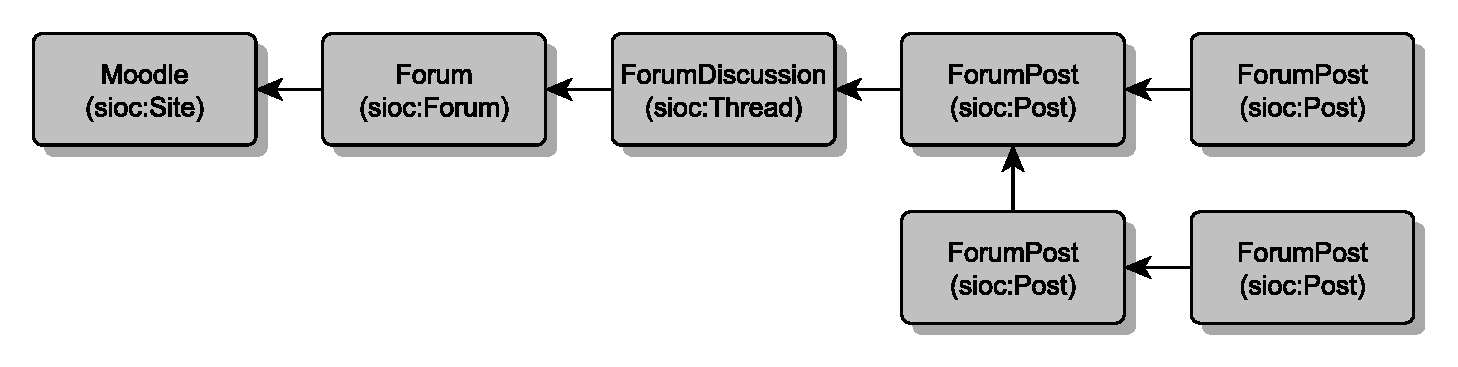
\includegraphics[
        width=\textwidth,
        keepaspectratio=true]
    {assets/images/mapping/moodle_sioc_mapping}
    \caption{Struktur von Moodle und Mapping nach SIOC}
    \label{fig:moodle_sioc_mapping}
\end{figure}

Für die Authentifizierung der Benutzerkonten werden für Moodle der entsprechende Benutzername und das Passwort benötigt. Diese werden als Credential für den \texttt{waa:Direct} Authentifizierungsmechanismus gespeichert, wie es in der Abbildung \ref{fig:moodle_useraccount_mapping} zu sehen ist. Für die Servicebeschreibung mit der Klasse \texttt{sioc:Service} aus dem SIOC Services Modul ist die Angabe der Adresse der Moodleinstanz mit der Eigenschaft \texttt{siocs:serviceEndpoint} für die API äußerst wichtig. Sie bestimmt den Endpunkt an dem die API-Abfragen gesendet werden.

\begin{figure}[ht]
    \centering
    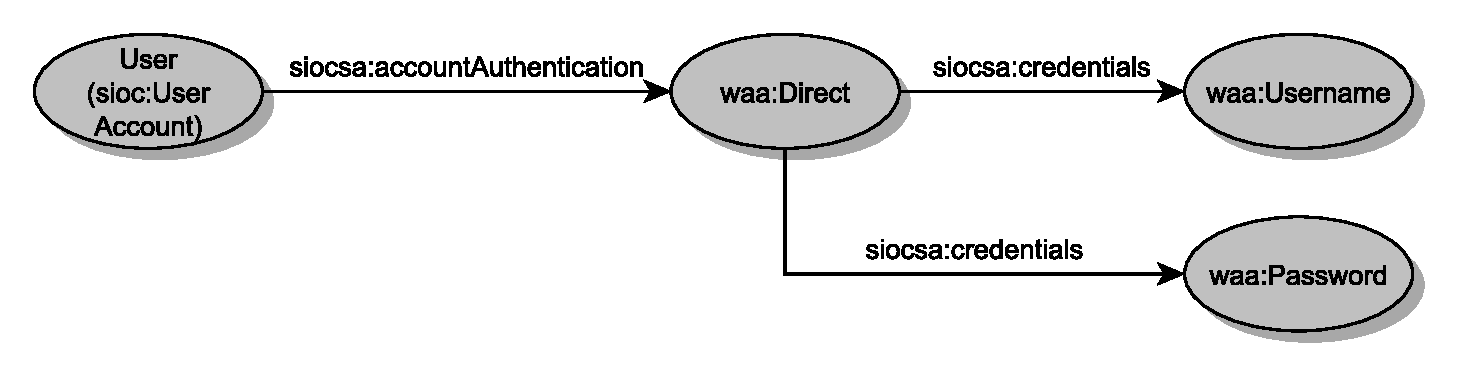
\includegraphics[
        width=0.95\textwidth,
        keepaspectratio=true]
    {assets/images/mapping/moodle_useraccount_mapping}
    \caption{Authentifizierungsdaten für Moodle in SIOC}
    \label{fig:moodle_useraccount_mapping}
\end{figure}

Die URIs für die Objekte der SIOC-Klassen für Moodle entsprechen den URIs der graphischen Weboberfläche, da SOAP keine expliziten URIs für Ressourcen besitzt. Das genaue Format ist in der Tabelle \ref{tbl:moodle_sioc_uris} beschrieben. Der Platzhalter \texttt{\{rootId\}} entspricht den Wert der Eigenschaft \texttt{siocs:serviceEndpoint} aus der Servicebeschreibung.

\begin{table}[ht]
    \centering
    \caption{Format der URIs für Moodle in RDF}
    \begin{tabular}{l|p{13cm}}
        \textbf{SIOC Klasse} & \textbf{URI-Format} \\ 
        \hline
        \texttt{sioc:Site} & \texttt{\{rootUri\}}\\
        \texttt{sioc:Service} & \texttt{\{rootUri\}/wspp}\\
        \texttt{sioc:UserAccount} & \texttt{\{rootUri\}/user/profile.php?id=\{userId\}} \\
        \texttt{sioc:Forum} & \texttt{\{rootUri\}/mod/forum/view.php?id=\{forumId\}} \\
        \texttt{sioc:Thread} & \texttt{\{rootUri\}/mod/forum/discuss.php?d=\{discussionId\}} \\
        \texttt{sioc:Post} & \texttt{\{rootUri\}/mod/forum/discuss.php?d=\{discussionId\}\#p\{postId\}} \\
    \end{tabular}
    \label{tbl:moodle_sioc_uris}
\end{table}

% subsubsection moodle_mapping_nach_sioc (end)

\subsubsection{Besonderheiten bei der Implementierung des MoodleConnectors} % (fold)
\label{ssub:herausforderungen_bei_der_implementierung_des_moodleconnectors}

Der Connector für Moodle war wohl einer der herausforderndsten bei der Implementieren von allen fünf Connectoren. Nicht nur weil erst nach mehreren Test sich herausstellte, dass die favorisierte REST-Schnittstelle von MoodleWS kein Schreiben von Beiträgen möglich macht, sondern dass auch die Java-Bibliothek moodlews\_ksoap2 so ihre kleinen Eigenheiten hat. 

Zuerst mussten die Klassen für moodlews\_ksoap2 komplett neu generiert werden, da die auf GitHub bereitgestellten Klassen nicht kompatibel zur aktuellsten WSDL-Datei des MoodleWS Plugins waren. Der passende Generator wird aber vom Entwickler gleich mitgeliefert und ist mit dem folgenden Befehl schnell erledigt.

\begin{lstlisting}[
    caption={Neugenerierung von moodlews\_ksoap2}\label{lst:neugenerierung_moodlews_ksoap2},
    captionpos=t]
    java  org.ksoap2.wsdl.WSDL2ksoap -p de.m0ep.moodlews.soap -o /tmp http://localhost/moodle/wspp/wsdl_pp2.php
\end{lstlisting}

Mit dem Parameter \enquote{-p} wir das Java-Package für die Java-Klassen festgelegt und mit \enquote{-o} der Ordner in dem die Klassen geschrieben werden. Die URI am Ende gibt den Pfad zur Datei \enquote{wsdl\_pp2.php} vom MoodleWS-Plugin an. Diese URI ist dann an die jeweilige Moodleinstanz anzupassen.

Eine sehr nervende Eigenheit von moodlews\_ksoap2 ist die Tatsache, dass Java-Exceptions und Gründe für Fehler gerne verschluckt und nicht weitergegeben werden. So ist es zum Beispiel unmöglich zu wissen, ob eine Operation aufgrund eines Netzwerkfehlers, eines abgelaufenen Sitzungsschlüssels oder falschen Daten fehlschlug. Aus diesem Grund wurde der Client von moodlews\_ksoap2 für den ClientManager (siehe Abschnitt \ref{sub:clientmanager}) in eine extra Klasse \texttt{Moodle2ClientWrapper} gepackt und um Mechanismen zur Fehlererkennung und Wiederherstellung des Clients erweitert. Alle Funktionsaufrufe des Clients wie \texttt{get\_all\_forums(\dots)} werden dazu zuerst in die Methode \texttt{call()} eines Objekts der Java-Schnittstelle \texttt{Callable<V>}\footnote{\url{http://docs.oracle.com/javase/7/docs/api/index.html?java/util/concurrent/Callable.html}} verpackt, so dass diese Funktion, ohne zu wissen um welche es sich genau handelt, mehrfach aufgerufen werden kann. Diese Objekt wird dann an die Methode \texttt{callMethod(\dots)} der Klasse \texttt{Moodle2ClientWrapper} übergeben. Diese Methode ruft zuerst die \texttt{call()}-Methode des Callable-Objekts auf und prüft ob ein gültiges Ergebnis zurückgegeben wurde. Dies ist der Fall wenn es ungleich \texttt{null} ist. Ist dies nicht der Fall, wird geschaut ob die Moodleinstanz erreichbar ist. Sollte hier alles in Ordnung sein, muss geschaut werden ob der Sitzungsschlüssel abgelaufen ist. Als Test reicht es hier aus zu testen, ob die Methode \texttt{get\_my\_id(\dots)} des moodlews\_ksoap2 Clients eine Zahl ungleich Null zurück gibt. Diese liefert die ID des aktuell angemeldeten Benutzers zurück und im Fehlerfall ist dieser gleich Null. Ist dieser Test positiv, also der Sitzungsschlüssel abgelaufen, wird versucht sich neu anzumelden und die Anfrage erneut ausgeführt. Ansonsten wird ein Fehler gemeldet.

Eine Funktion mit der nur ein Beitrag mit einer bestimmten ID abgefragt werden könnte fehlt ebenfalls. Wenn nur ein Beitrag geladen werden soll, müssen zunächst alle innerhalb des selben Threads angefordert und diese nach dem passenden Beitrag durch werden. 

Als ungewöhnlich kann auch der Inhalt der Klasse \texttt{ForumDiscussionRecord} bezeichnet werden, welche die Informationen zu einen Thread enthält. Normalerweise würde man erwarten, dass die Methode \texttt{getId()} die ID des Threads zurück geben wird. Doch stattdessen entspricht der Wert der ID des ersten Beitrags dieses Threads. An die richtige ID kommt man erst heran, wenn man sich mit der Methode \texttt{getPost()} ein Objekt des ersten Beitrags holt und darin den Rückgabewert von \texttt{getDiscussion()} benutzt.

% subsubsection herausforderungen_bei_der_implementierung_des_moodleconnectors (end)

% subsection moodle_connector (end)

\subsection{CanvasConnector} % (fold)
\label{sub:canvas_connector}

Für den Zugriff auf die Lernplattform Canvas über SIOC wurde der \emph{CanvasConnecor} implementiert. Wie schon bei Moodle war das Mapping nach SIOC aufgrund der Forenstruktur unkompliziert. Das gleiche gilt auch für die bereitgestellte REST-API die einwandfrei funktionierte. Da aber noch keine API für Java existierte, musste erst eine eigne entwickelt werden. Diese unterstützt leider noch nicht alle Ressourcen von Canvas, ist aber für die Zwecke des CanvasConnectors erst einmal völlig ausreichend. 

% \begin{itemize}
%     \item relativ neues LMS
%     \item super Bedienung
%     \item super REST API
%     \item keine Java API
%     \item rudimentäre Eigenentwicklung einer Java API, Funktionsweise ähnlich  G+
%     \item viel API Funktionen wohl nicht extern nutzbar (UserProfil lesen, vll. Falsche Berechtigung -> test nötig)
% \end{itemize}

\subsubsection{Canvas REST-API} % (fold)
\label{ssub:canvas_api}

Der öffentliche Zugriff auf die Daten der Lernplattform Canvas basiert auf einer REST-API und OAuth 2.0 zur Autorisierung. Die Adresse, über die auf die API zugegriffen werden kann, besteht aus der URI für die verwendete Canvasinstanz (\texttt{\{rootUri\}}) gefolgt von dem Pfad \enquote{/api/v1}. Für die Demoinstanz von Instructre würde dies der URI \texttt{https://canvas.instructure.com/api/v1} entsprechen. An diese können dann weitere Pfade für den Zugriff auf die einzelnen Ressourcen angehängt werden. Zur Autorisierung wird von OAuth nur der Accesstoken benötigt, der bei der REST-Abfrage als HTTP Authorization Header mitgeschickt wird. Listing \ref{lst:canvas_authorization_header} zeigt eine Beispielanfrage und Angabe des Accesstokens mit dem Programm \emph{curl}\footnote{\url{http://curl.haxx.se/}}. Der Platzhalter \texttt{\{accessToken\}} muss dann natürlich erst durch einen validen Accesstoken ersetzt werden. Diesen kann jeder Benutzer in seinem Canvas-Profil unter \enquote{Settings} und im Abschnitt \enquote{Approved Integrations} selbst erstellen. Die Angabe von ClientId und ClientSecret sind nicht nötig.

\begin{lstlisting}[
    caption={Canvas Authorization Header}\label{lst:canvas_authorization_header},
    captionpos=t]
curl -H "Authorization: Bearer {accessToken}" https://canvas.instructure.com/api/v1/courses
\end{lstlisting}

Als Datenformat für die zurückgelieferten Daten wird von Canvas auf JSON gesetzt. Für die Verwendung von POST und PUT Operationen, zum Schreiben nach Canvas, können die Daten entweder im \emph{HTML Form Encoding}\footnote{\url{http://www.w3.org/TR/html4/interact/forms.html\#h-17.13.4}} Standard oder ebenfalls in JSON angegeben werden. 

Da einige Abfragen eine Liste von Ergebnissen zurückliefern und diese möglicher Weise sehr lang werden können, teilt Canvas diese Listen auf mehrere Seiten auf, die jede einzeln abgefragt werden müssen. Für jede Seite schickt Canvas mehrere URIs als \emph{HTTP Link Header}\footnote{\url{http://www.w3.org/Protocols/9707-link-header.html}} der Antwort mit. Diese URIs erhalten zusätzlich noch ein Attribut \texttt{rel} mit, das beschreibt in welcher Relation die URI zu dieser Seite steht.  Als Wert für diese Relation können \enquote{current} für eine URI auf die aktuelle, \enquote{next} auf die nächste, \enquote{prev} auf die vorherige, \enquote{first} auf die erste und \enquote{last} für eine URI auf die letzte Seite vorkommen. Um also die nächste Seite vom Ergebnis zu bekommen, muss eine neue REST-Abfrage mit der URI aus dem Link mit der Relation \enquote{next} ausgeführt werden. Fehlt eine URI mit dieser Relation, ist die letzte Seite des Ergebnisses erreicht. 

% subsubsection canvas_api (end)

\subsubsection{CanvasLMS4J} % (fold)
\label{ssub:canvaslms4j}

Ein Problem mit der API von Canvas war es, dass es zwar eine gute REST-basierte Anbindung gab, aber noch keine Bibliothek, um sie mit der Programmiersprache Java anzusprechen. Es musste also erst eine eigne Java API  entwickelt werden, die den Namen \emph{CanvasLMS4J} (Kurzform für \enquote{Canvas LMS API für Java}) bekam. Inspiriert wurde diese entwickelte API von Teilen aus RestFB und der Google+ API die später noch vorgestellt werden.

Anhand der für die REST-API verwendeten URIs ist auffällig, dass die einzelnen Bestandteile aufeinander aufbauen. Zum Beispiel ist der Ablauf für den REST-Zugriff auf DiscussionTopics in Gruppen und Kursen der gleiche, nur der Anfang der verwendeten URIs unterscheidet sich. Aus diesem Grund wurden die einzelnen Ressource (Course, Groupe, DiscussionTopic, Entries, ...) als einzelne Endpunkte implementiert, die sich von der Klasse \texttt{IEnpoint} ableiten. Jeder Endpunkt kann einen Eltern-Endpunkt haben, wobei sich die endgültige URI für die REST-Abfrage aus dem Pfad des Eltern-Endpunktes und dem des aktuellen Endpunktes zusammensetzt. Zur Verdeutlichung sei hier die URI \texttt{https:\{canvasUri\}/api/v1/courses/1/discussion\_topics} als Demonstration genannt. Sie besteht aus den statischen Teil \texttt{https:\{canvasUri\}/api/v1/} der den Ort für die verwendete Canvasinstanz angibt. Darauf folgt ein Kurs als erster Endpunkt mit der Kurs-ID \enquote{1}. Für diesen Kurs sollen nun alle Diskussionen abgefragt werden. Dies geschieht durch die Angabe des zweiten Endpunktes \texttt{/discussion\_topics}. der Pfad \enquote{/courses/1} bildet hier also den Eltern-Endpunkt von \texttt{/discussion\_topics}. Sollen aber nun alle Diskussionen in einer Gruppe abgefragt werden, reicht es aus den Kurs-Endpunkt durch einen Gruppen-Endpunkt auszutauschen: \texttt{https:\{canvasUri\}/api/v1/groups/42/discussion\_topics}.

\begin{figure}[p]
    \centering
    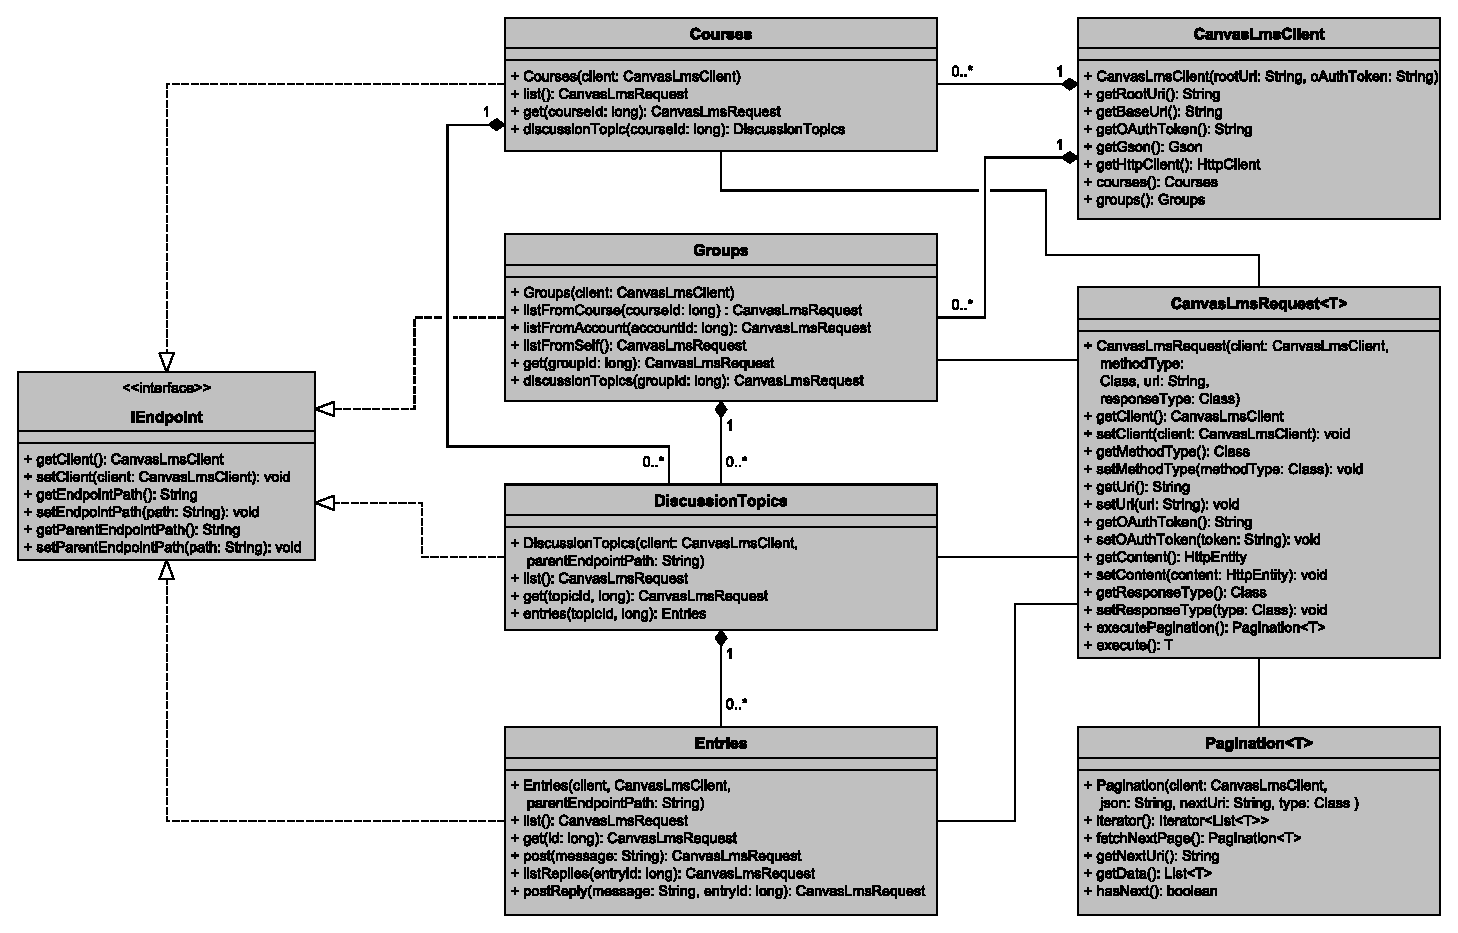
\includegraphics[
        width=\textwidth,
        keepaspectratio=true,]
    {assets/images/canvaslms4j_uml_classdiagramm}
    \caption{UML Klassendiagramm von CanvasLMS4J}
    \label{fig:canvaslms4j_uml_classdiagram}
\end{figure} 

Ausgangspunkt für CanvasLMS4J ist der Client mir der Klasse \texttt{CanvasLmsClient} (siehe Abbildung \ref{fig:canvaslms4j_uml_classdiagram}). Über sie werden alle Endpunkte verwaltet, die keinen Eltern-Endpunkt besitzen. Bei der Erzeugung eines Objektes dieser Klasse, werden ihr die URI zur verwendenden Canvasinstanz (ohne \enquote{\texttt{/api/v1}}) und der Accesstoken des Benutzerkontos übergeben. Im aktuellen Stadium können von einem Client aus nur auf Endpunkte für Kurse oder Gruppe zugegriffen werden.

Endpunkte können dann mit die Klasse \texttt{CanvasLmsRequest} REST-Anfragen an die Canvas API stellen. Hierzu verwendet CanvasLMS4J die \emph{HttpClient}\footnote{\url{http://hc.apache.org/httpclient-3.x/}} Bibliothek von Apache mit der einzelne HTTP-Operationen ausgeführt werden können. Um die im JSON-Format zurück gelieferten Antworten von Canvas in Java verwenden zu können, wird auf die Funktionen der von Google entwickelten \emph{Gson}\footnote{\url{https://code.google.com/p/google-gson/}} Bibliothek zurückgegriffen. Sie erlaubt es Java Objekte in das JSON-Format zu konvertieren und genauso aus Daten in JSON ein Java-Objekt zu erzeugen (eine passende Klasse muss aber vorhanden sein). Dadurch verringert sich der Aufwand für das Verarbeiten der Daten von Canvas auf das Erstellen der entsprechenden Java-Klassen. CanvasLmsRequests können mit zwei verschiedenen Methoden ausgeführt werden. Die erste \texttt{execute()} wird dazu verwendet, wenn die REST-Abfrage nur die Rückgabe eines Objektes zur Folge hat. Also zum Beispiel, wenn nur die Daten eines bestimmten Kurses abgefragt werden sollen. Die zweite Methode ist \texttt{executePagination()}. Diese Methode dient für Abfragen die eine in Seiten aufgeteilte Liste von Ergebnissen zurückliefern und gibt für eine einfache Handhabbarkeit ein Objekt der Klasse \texttt{Pagination} zurück. 

Diese Klasse Pagination ist nach dem Iterator-Muster aufgebaut und liefert vom kompletten Ergebnis bei jedem Iterationsschritt eine einzelne Seite zurück. Diese Seite enthält dann je eine Teilliste der angefragten Objekte. Ist eine Seite fertig ausgelesen, holt Pagination über eine vorgegeben REST-Abfrage die nächste Seite. Dies geschieht solange bis keine Seiten mehr geladen werden können oder das Programm das Lesen abbricht.

\begin{lstlisting}[
    caption={CanvasLMS4J Beispielprogramm}\label{lst:canvaslms4j_beispiel},
    captionpos=t]
CanvasLmsClient client = new CanvasLmsClient(
                "https://canvas.instructure.com",
                "7~LUpV7B3lJY...");

Pagination<DiscussionTopic> discussionPages = client.courses()
    .discussionTopics( 798152 )
    .list()
    .executePagination();

for ( List<DiscussionTopic> discussions : discussionPages ) {
    for ( DiscussionTopic discussion : discussions ) {
        System.out.println( discussion );
    }
}

\end{lstlisting}

In Listing \ref{lst:canvaslms4j_beispiel} ist ein Beispiel für die Anwendung der CanvasLMS4J API zu sehen. In den ersten drei Zeilen wird eine neuer CanvasLmsClient für die Canvasinstanz auf \texttt{https://canvas.instructure.com} und einem AccessToken erstellt. Als nächstes soll für einen Kurs mit der ID \enquote{798152} alle Diskussionen aufgelistet werden. Mit dem Aufruf der Methode \texttt{courses()} des Clients wir der Endpunkt für die Kurse und von diesem aus der Endpunkt für die Diskussionen im Kurs \enquote{798152} abgefragt. In der siebten Zeile wird die Art der Abfrage genauer festgelegt. Da eine Liste aller Diskussionen gesucht ist, wird die Methode \texttt{list()} aufgerufen die ein CanvasLmsRequest-Objekt für die gewünschte Abfrage erstellt. Da die Antwort aus mehrere Objekten mit der Beschreibung der einzelnen Diskussionen besteht, wird die Anfrage in Zeile 8 mit der Methode \texttt{executePagination()} ausgeführt. Die einzelnen Seiten des Ergebnisses werden dann in der zehnten Zeile mit einer For-Schleife durchlaufen. Das nachladen der Seiten erfolgt dabei automatisch durch die Pagination-Klasse. Jede Seite besteht nun aus einer Liste mit den Beschreibung der Diskussionen in einem \texttt{DiskussionTopic}-Objekt, welche dann wiederum in einer weiteren Schleife ausgegeben werden.

% subsubsection canvaslms4j (end)

\subsubsection{Mapping von Canvas nach SIOC} % (fold)
\label{ssub:canvas_sioc_mapping}

Die Struktur von Canvas ist der von Moodle sehr ähnlich (siehe Abbildung \ref{fig:canvas_sioc_mapping}), nur dass es explizit keine Foren gibt sondern die Diskussionen innerhalb der Kurse stattfindet. Demzufolge kann ein Kurs (\texttt{Course}) der SIOC-Klasse \texttt{sioc:Forum} zugeordnet werden. Dies gilt ebenfalls für Gruppen, in denen separate Diskussionen geführt werden können. Die Diskussionsthemen in Canvas werden durch die Klasse \texttt{DiscussionTopic} modelliert und entspricht \texttt{sioc:Thread} . Die Klasse für Beiträge in Canvas ist \texttt{Entry} und ist entweder ein Kommentar auf den ersten Beitrag einer Diskussion oder eins auf dessen Kommentare. Die SIOC-Klasse für einen Entry entspricht demzufolge \texttt{sioc:Post}.
 
\begin{figure}[ht]
    \centering
    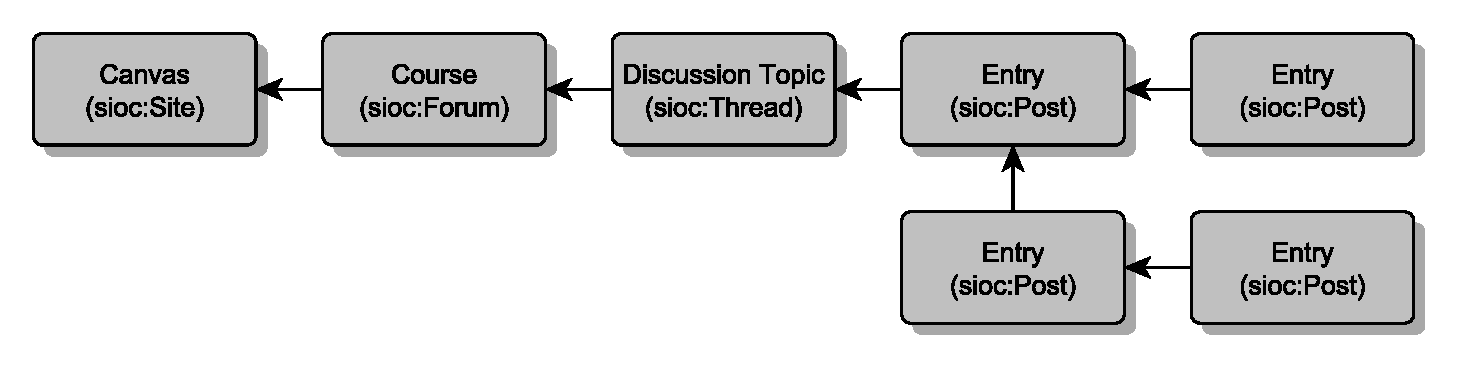
\includegraphics[
        width=0.9\textwidth,
        keepaspectratio=true]
    {assets/images/mapping/canvas_sioc_mapping}
    \caption{Struktur von Canvas und Mapping nach SIOC}
    \label{fig:canvas_sioc_mapping}
\end{figure}

Zum Benutzen der REST-API von Canvas muss eine Accesstoken für den betreffenden \texttt{sioc:UserAccount} des Benutzerkontos vorliegen. Wie in Abbildung \ref{fig:canvas_useraccount_mapping} wird der Accesstoken dem \texttt{sioc:UserAccount} mit \texttt{siocsa:accountAuthentication} als Credential der Klasse \texttt{waa:OAuth} mitgegeben. In der Servicebeschreibung ist wieder die Angabe von \texttt{siocs:serviceEndpoint} mit der Adresse der Canvasinstanz für die API Voraussetzung für den Betrieb des CanvasConnectors.

\begin{figure}[ht]
    \centering
    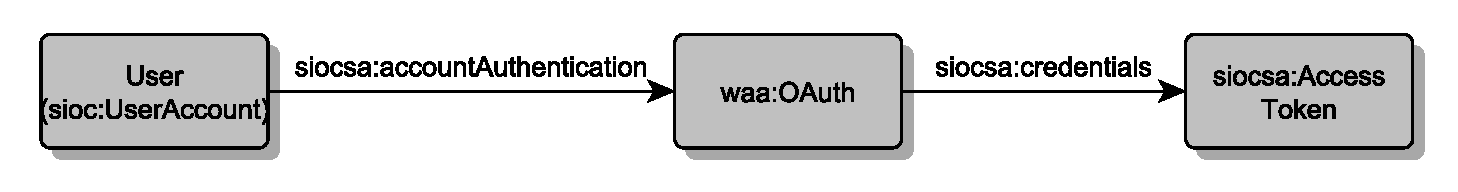
\includegraphics[
        width=\textwidth,
        keepaspectratio=true]
    {assets/images/mapping/canvas_useraccount_mapping}
    \caption{ Authentifizierungsdaten für Canvas in SIOC}
    \label{fig:canvas_useraccount_mapping}
\end{figure}

Die URIs für RDF bei Canvas wurden so gewählt, dass sie den URIs für die REST-Abfragen entsprechen. An ihnen ist sehr leicht zu erkennen, wo die Ressource sich innerhalb der Canvasstruktur befindet, da sie aufeinander aufbauen. Das einzige Problem liegt nur in der URI für den Startbeitrag einer Diskussion, da dieser nur innerhalb des DiskusionTopics existiert und keine eigene ID besitzt. Aus diesem Grund wurde für die URI des Startbeitrags die Zusammensetzung aus der URI eines DiscussionTopics mit angehängten Fragment \enquote{\texttt{\#discussion\_topic}} gewählt. Dieser Zusatz wurde nicht zufällig ausgewählt. Die ID \enquote{\texttt{discussion\_topic}} wird von Canvas innerhalb der HTML-Darstellung für genau diesen Beitrag verwendet. 

\begin{table}[ht]
    \centering
    \caption{Format der URIs für Canvas in RDF}
    \begin{tabular}{l|p{13cm}}
        \textbf{SIOC Klasse} & \textbf{URI-Format}\\ 
        \hline
        \texttt{sioc:Site} & 
        \texttt{\{rootUri\}} \\

        \texttt{sioc:Service} & 
        \texttt{\{rootUri\}/api/v1} \\

        \texttt{sioc:UserAccount} & 
        \texttt{\{rootUri\}/api/v1/users/\{userId\}/profile} \\

        \texttt{sioc:Forum} & 
        \texttt{\{rootUri\}/api/v1/courses/\{courseId\}} \emph{oder} \newline  \texttt{\{rootUri\}/api/v1/groups/\{groupId\}} \\

        \texttt{sioc:Thread} & 
        \texttt{\{forumUri\}/discussion\_topics/\{topicId\}} \\

        \texttt{sioc:Post} & 
        \texttt{\{threadUri\}/entries/\{entryId\}} \emph{oder} \newline \texttt{\{threadUri\}\#discussion\_topic} \\
    \end{tabular}
    \label{tbl:canvas_uri_platzhalter}
\end{table}

% subsubsection canvas_sioc_mapping (end)

% subsection canvas_connector (end)

\subsection{FacebookConnector} % (fold)
\label{sub:facebook_connector}

Dieser Abschnitt beschreibt, wie man auf die Daten von Facebook zugreifen kann, um einen FacebookConnector zu entwickeln. Zuerst wird dazu die \emph{Graph API} von Facebook vorgestellt. Danach erfolgt eine Beschreibung der Java-Bibliothek \emph{RestFB}, welche das Verwenden der Graph API aus Jave heraus ermöglicht. Zum Abschluss folgt noch das Mapping der Facebook Ressourcen in die entsprechenden SIOC-Klassen. 

% \begin{itemize}
%     \item REST API + JSON
%     \item keine offizielle Java API für Desktop -> Web + Mobile only
%     \item GraphAPI, Facebook Query Language
%     \item OAuth 2.x
%     \begin{itemize}
%         \item kein Refreshtoken
%         \item Token Haltbarkeit 2h (2 Monate, wen extended)
%         \item token nur über webbrowser
%     \end{itemize}
%     \item RestFB alternative Java API für die REST Schnittstelle der GraphAPI
%     \item Typ der zurückgelieferten Daten nicht anhand der URI erkennbar, häufig erst durch Angabe von \emph{metadata=1}
%     \item beim herunterladen einzelner Posts nicht immer erkennbar wo sie geschrieben wurden
% \end{itemize}

\subsubsection{Facebook Graph API} % (fold)
\label{ssub:facebook_graph_api}

Der primäre Weg an die von Facebook gespeicherten Daten zu gelangen, geht über die \emph{Graph API} (siehe. \cite{FacebookGraphAPI}). Sie erlaubt einen REST-basierten Zugriff auf den sogenannten \emph{Social Graph} von Facebook. Dieser Graph enthält alle Beziehungen die ein Person auf Facebook zwischen anderen Personen, Gruppen, Seiten, Beiträge, Fotos und so weiter besitzt. Der einfachste Weg zum Kennenlernen der Graph API ist der \emph{Graph API Explorer}\footnote{\url{https://developers.facebook.com/tools/explorer}}. Er ist eine Onlineanwendung für REST-Abfragen an die Graph API, um schnell etwas auszuprobieren.

Jede Ressource im Social Graph von Facebook hat seine eigene, eindeutige ID. Die URI für den REST-Zugriff auf eine Ressource besteht aus \texttt{https://graph.facebook.com/} gefolgt von der ID und optionalen Parametern. Dies macht die Form der URIs zwar sehr einheitlich, aber es ist so unmöglich anhand der URI herauszufinden welcher Typ von Ressource sich dahinter befindet. Dies widerspricht zwar nicht die am Anfang von Kapitel \ref{cha:eigener_ansatz_social_online_community_connectors_socc_} beschreiben Prinzipien von Berners-Lee macht aber die spätere Verarbeitung etwas komplizierter. 

\paragraph{Graph API Datenformat} % (fold)
\label{par:graph_api_datenformat}

Als Datenformat setzt Facebook mit der Graph API auf das weit verbreitete JSON-Format. Neben den eigentlichen Daten enthalten Ressourcen noch Verbindungen zu anderen Ressourcen. Diese Verbindungen werden \enquote{Connections} genannt. Um zu lesen welche Connections eine Ressource besitzt, muss bei der Abfrage der Parameter \texttt{metadata=1} angehängt werden. Ist dies geschehen, enthalten die JSON-Daten einen neuen Eintrag \texttt{metadata} und darin unter dem Eintrag \texttt{connections} eine Liste der vorhandenen Connections. Die wichtigsten Connections für den FacebookConnector sind \texttt{feed} und \texttt{comments}. Die Connection \texttt{feed} sagt über die Ressource aus, dass sie eine Liste von Beiträgen enthält und in sie Beiträge geschrieben werden können. Das könnte zum Beispiel die Wall einer Person oder die einer Gruppe sein. Dahingegen zeigt die Connection \texttt{comments} an, dass die betreffende Ressource Kommentare enthält und auch kommentiert werden kann. Um die Beiträge eines Feeds lesen zu können, muss nur die URI der Ressource mit dem Pfad \texttt{/feed} erweitert werden $\rightarrow$ \texttt{http:/graph.facebook.com/me/feed}. Die ID \enquote{\texttt{me}} ist dabei ein spezielle ID, die sich auf den aktuell angemeldete Benutzer bezieht. Möchte man nun nicht alle Daten einer Ressource abfragen, sondern zum Beispiel nur den Name und das Datum der letzten Änderung, kann der Parameter \enquote{\texttt{fields}} der URI hinzugefügt werden. Als Wert wird dann eine Liste mit den Namen der gesuchten Datenfelder angegeben, wobei jeder Name durch ein Komma getrennt wird. 

% paragraph graph_api_datenformat (end)

\paragraph{Facebook Login} % (fold)
\label{par:facebook_login}

Die Graph API verwendet zur Autorisierung für die Abfragen OAuth 2.0. Auch \emph{Facebook Login}\footnote{\url{https://developers.facebook.com/docs/facebook-login/}} genannt. Accesstoken sind bei Facebook nur für zwei Stunden gültig. Es ist aber möglich einen \emph{Long-Lived Accesstoken}\footnote{\url{https://developers.facebook.com/docs/facebook-login/access-tokens/}} zu erstellen, der zwei Monate gültig ist. Ist ein Accesstoken irgendwann abgelaufen, muss vom Benutzer ein neuer erstellt werden. Da aber die Graph API hauptsächlich nur für Webanwendungen gedacht ist, kann dies ein Desktopprogramm nur mit dem Umweg über einen Internetbrowser machen. Für das Anlegen eines neuen Accesstokens werden vom Programm eine OAuth 2.0 ClientID und das ClientSecret benötigt. Diese bekommt man von Facebook, wenn man für sein Programm auf der Webseite \url{https://developers.facebook.com/apps} eine \enquote{App} anlegt. Die Daten befinden sich dann in den \enquote{Einstellungen} unter \enquote{Grundlegendes} und werden dort \enquote{App ID} und \enquote{App Secret} genannt.

Jeder Accesstoken hat nur Zugriff auf bestimmte Bereiche der Graph API, die beim Erstellen des selbigen als \enquote{Permission}\footnote{\url{https://developers.facebook.com/docs/reference/login/\#permissions}} (engl. für Berechtigungen), beziehungsweise von OAuth 2.0 \enquote{Scope} (engl. für Geltungsbereich) genannt, angegeben werden muss. Es ist absolut wichtig diese Berechtigungen auch in den App-Einstellungen unter \enquote{Berechtigungen} anzugeben. Ohne diese Angabe verweigert Facebook das Verwenden der dazugehörigen Ressourcen. Die für SOCC wichtigen Berechtigungen sind in der Tabelle \ref{tbl:socc_facebook_persmissons} beschrieben.

\begin{table}[ht]
    \centering
    \caption{Für SOCC wichtige Facebook Berechtigungen}
    \begin{tabular}{r|p{10cm}}
        \textbf{Berechtigung} & 
        \textbf{Beschreibung} \\ 
        \hline
        \textit{read\_stream} & 
        Lesen von Beiträgen und Kommentaren eines Benutzers. \\
        \textit{publish\_actions} & 
        Schreiben von Beiträgen und Kommentarten für einen Benutzer. \\
        \textit{user\_groups} & 
        Zugriff auf die Liste der beigetretenen Gruppen eines Benutzers.
    \end{tabular}
    \label{tbl:socc_facebook_persmissons}
\end{table}

Um nun einen Accesstoken für einen Benutzer zu Erstellen, muss in einen Internetbrowser folgende URI eingegeben werden:

\begin{lstlisting}[numbers=none, belowskip=-18pt]
https://www.facebook.com/dialog/oauth?client_id={appId}
    &redirect_uri={redirectUri}&responseType=code&scope={scopeList}.
\end{lstlisting}

Anstatt des Platzhalters \texttt{\{appId\}}, muss dann die oben angesprochene ClientID beziehungsweise App ID eingetragen werden. Mit dem Parameter \texttt{redirect\_uri} wird bei dieser URI eine Adresse angegeben, auf die der Internetbrowser nach der Anfrage mit der Antwort umgeleitet wird. Dies kann die Adresse eines externen Webservers oder die eines Webservers den die Anwendung nur für diesen Zweck laufen lässt sein. Einen solchen Webserver kann man mit der Jetty\footnote{\url{http://www.eclipse.org/jetty}} Bibliothek für Java erstellen und würde dann als \texttt{redirect\_uri} die URI \texttt{http://localhost:\{port\}/} angeben. Der Parameter \texttt{responseType=code} besagt, dass diese Anfrage einen Code zurück liefert mit dem dann der eigentliche AccessToken abgeholt werden kann. Dies ist der Standardweg. Mit dem letzten Parameter \texttt{scope} können dann noch die oben erwähnten Berechtigungen übergeben werden, wobei alle durch eine Komma getrennt hintereinander zu schreiben sind. Wird dann diese URI im Browser aufgerufen, wird er danach bei Erfolg auf die Adresse \texttt{{redirectUri}?code=\{code\}} umgeleitet. Der Platzhalter \texttt{\{code\}} würde dann einen zufälligen Code darstellen, mit dem über eine weitere Anfrage mit der folgenden URI der Accesstoken geholt werden kann:

\begin{lstlisting}[numbers=none, belowskip=-18pt]
https://www..facebook.com/oauth/access_token?client_id={appId}
    &redirect_uri={redirectUri}&client_secret={appSecret}&code={code}
\end{lstlisting}

Der Platzhalter \texttt{\{appId\}} und \texttt{\{appSecret\}} entsprechen wieder der ClientID und ClientSecret. Bei dieser URI ist es sehr wichtig, dass \texttt{\{redirectUri\}} den selben Wert hat, wie er weiter oben schon einmal angegeben wurde. Für \texttt{\{code\}} muss dann noch der oben zurückgeliefert Code angegeben werden. Für diese Abfrage ist aber kein Internetbrowser mehr nötig. Als Antwort wird dem Programm dann die Daten \texttt{access\_token=\{accessToken\}\&expires=\{secondsTilExpiration\}} zurück geliefert. Der Wert des Parameters \texttt{access\_token} ist der gewollte Accesstoken und der Wert von \texttt{expires} ist die Haltbarkeit des Accesstokens in Sekunden.

Soll nun die Haltbarkeitsdauer des Tokens auf zwei Monate verlängert werden muss eine neue Anfrage mit der folgende URI gemacht werden:

\begin{lstlisting}[numbers=none, belowskip=-18pt]
https://www.facebook.com/oauth/access_token?grant_type=fb_exchange_token
    &client_id={appId}&client_secret={app-secret}
    &fb_exchange_token={accessToken}
\end{lstlisting} 

Die Werte für die einzelnen Parameter dürften nun offensichtlich sein. Als Antwort kommt dann ein Accesstoken mit verlängerter Haltbarkeit zurück. Dabei kann es passieren, dass er genau so aussieht wie der alte, was aber kein Problem darstellt.

% paragraph facebook_login (end)

% subsubsection facebook_graph_api (end)

\subsubsection{RestFB} % (fold)
\label{ssub:restfb}

Facebook selber bietet direkt keine API für die Verwendung der Graph API in Desktopprogrammen an. Speziell für die Programmiersprache Java existiert von Facebook nur eine API für das mobile Betriebssystem Android\footnote{\url{https://developers.facebook.com/docs/android/}}. Als Alternative dazu kann die \emph{RestFB}\footnote{\url{ http://restfb.com/}} Java-Bibliothek von Mark Allen verwendet werden. RestFB bietet dabei die Möglichkeit von Java aus die Graph API von Facebook zu benutzen. Eine Abfrage könnte wie in Listing \ref{lst:restfb_beispielprogramm} aussehen.

\begin{lstlisting}[
    caption={RestFB Beispielprogramm}\label{lst:restfb_beispielprogramm},
    captionpos=t]
FacebookClient client = new DefaultFacebookClient(USER_ACCESS_TOKEN);

User user = client.fetchObject("me", User.class);
System.out.println("User name: " + user.getName());

Connection<Post> myFeed = client.fetchConnection("me/feed", Post.class);
for (List<Post> feedPage : myFeed){
    for (Post post : feedpage){
        System.out.println("Post: " + post);
    }
}
\end{lstlisting} 

In Zeile Eins wird eine Objekt der Klasse \texttt{FacebookClient} mit einem Accesstoken als Parameter erstellt, über dem die Methoden für die Abfragen aufgerufen werden können. Die Zeile 3 zeigt eine solche Abfrage nach den Benutzerdaten für den aktuell angemeldeten Benutzer mit der speziellen ID \enquote{me}. Der Anfangsteil der URI für die Graph API \texttt{https://graph.facebook.com} muss dabei weggelassen werden. Zurück gegeben wird ein Objekt der Klasse \texttt{User} und über dies wird dann der Benutzername ausgegeben. Die Angabe der Klasse mit \texttt{User.class} ist ebenfalls essenziell. So weiß RestFB in welche Klasse es die von der Graph API zurückgelieferten JSON-Daten konvertieren soll. Zeile 6 zeigt noch wie man an die Daten einer Connection, hier der Beiträge auf der Wall des aktuellen Benutzers, gelangen kann. Enthält eine Antwort eine Liste mit zu vielen Einträgen, wird die Antwort auf mehrere Seiten aufgeteilt und ein Verweis auf die nächste Seite der aktuellen Seite mitgegeben. Die Klasse \texttt{Connection} sorgt dann alleine dafür, dass die neue Seite gelesen wird, wenn die alte abgearbeitet wurde. Die erste for-Schleife in Zeile 7 iteriert dann über alle vorhandenen Seiten und die zweite in Zeile 8 über alle Einträge auf der aktuellen Seite.

\begin{lstlisting}[
    caption={RestFB: Schreiben von Beiträgen auf eine Wall}\label{lst:restfb_write_post},
    captionpos=t]
FacebookType result = client.publish(
        userId + "/feed,
        FacebookType.class,
        Parameter.with("message", "Tolles Wetter heute \\o/"));
\end{lstlisting}

Beiträge können bei Facebook nur an Ressourcen geschrieben werden, die eine \enquote{feed} oder \enquote{comment} Connection haben. In Listing \ref{lst:restfb_write_post} ist zu sehen wie ein neuer Beitrag auf die Wall eines Benutzers geschrieben werden kann. Zu diesem Zweck enthält der Client aus RestFB die Methode \texttt{publish(\dots)} zum Schreiben von Daten in Ressourcen. Das erste Argument ist die Zielressource, die in Zeile 2 aus der ID des Benutzers gefolgt von einen \enquote{/} und dem Namen der Connection, hier \enquote{feed}, besteht. Da \texttt{publish(\dots)} bei Erfolgt die ID des erstellten Beitrags zurückliefert, wird als Klasse für das erwartete Ergebnis die Basisklasse \texttt{FacebookType} angegeben. Als letztes muss noch der Inhalt des Beitrags festgelegt werden. Dies geschieht nicht im JSON-Format, sondern wird als Parameter in der URI für die HTTP-POST-Operation angegeben. RestFB bietet dazu die Klasse \texttt{Parameter} an, mit der ein Parameter \enquote{message} und dem Inhalt des Beitrags als Wert erzeugt wird.

Facebook erlaubt mit der Graph API das Schreiben von Beitragen auf die Wall eines Benutzers nur, wenn das beim Schreiben verwendete Benutzerkonto mit dem der Wall übereinstimmt. Also das stellvertretende Schreiben auf eine fremde Wall ist nicht möglich. Diese Einschränkung gilt aber nicht für Walls von Facebook-Gruppen.

% subsubsection restfb (end)

\subsubsection{Mapping von Facebook nach SIOC} % (fold)
\label{ssub:facebook_mapping_nach_sioc}

Die Struktur von Facebook baut auf Walls von Benutzern, Gruppen und Facebook-Seiten auf. Darin können Beiträge geschrieben und diese kommentiert werden. Solch eine Wall entspricht der SIOC-Klasse \texttt{sioc:Forum}. Diese enthält aber keine weiteren Threads, sondern die Beiträge und Kommentare als \texttt{sioc:Post} Objekte. Abgesehen von Facebook-Seiten können Kommentare in Facebook zum aktuellen Zeitpunkt nicht kommentiert werden. Abbildung \ref{fig:facebook_sioc_mapping} zeigt dies noch einmal graphisch mit einer Gruppen-Wall als Beispiel.

\begin{figure}[!ht]
    \centering
    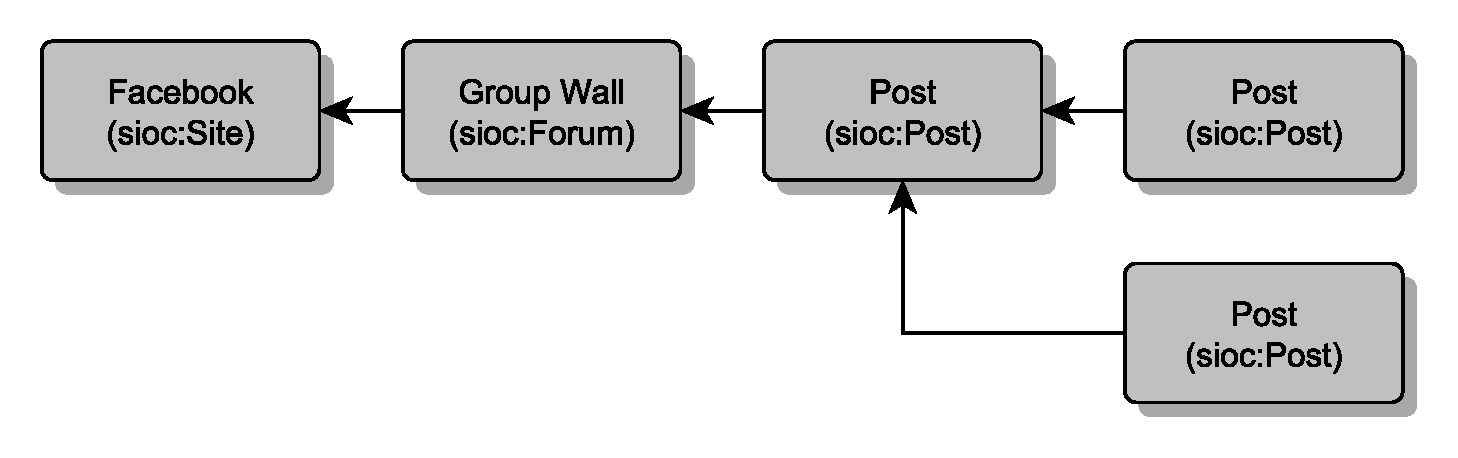
\includegraphics[
        width=.8\textwidth,
        keepaspectratio=true]
    {assets/images/mapping/facebook_sioc_mapping}
    \caption{Struktur von Facebook und Mapping nach SIOC}
    \label{fig:facebook_sioc_mapping}
\end{figure}

Wie weiter oben erklärt, verwendet Facebook für die Autorisierung der Abfragen in der Graph API OAuth 2.0. Die Benutzerkonten, die für das stellvertretende Schreiben verwendet werden sollen, müssen also einen Accesstoken für das Konto enthalten. Das gleiche gilt für die Servicebeschreibung für die Graph API mit der \texttt{siocs:Service} Klasse. Die Eigenschaft \texttt{siocsa:serviceAuthentication} zeigen auf ein Objekt der Klasse \texttt{waa:OAuth} das die ClientID und das ClientSecret enthält, wie es in der Abbildung \ref{fig:facebook_useraccount_mapping} zu sehen ist.

Die in RDF verwendeten URIs für die Klassen \texttt{sioc:Post} und \texttt{sioc:UserAccount} von Facebook bekommen das Format \texttt{https://graph.facebook.com/\{facebookId\}}, wobei \texttt{\{facebookId\}} der ID der Ressource entspricht. Ausnahme bildete die URIs für die Klasse \texttt{sioc:Forum}. Da die ID eines Benutzers sowohl für sein Konto als auch für seine Wall stehen würden, wird der URI für die Wall noch der Pfad \enquote{\texttt{/feed}} angehängt. Die URI \\texttt{https://graph.facebook.com/\{facebookId\}/feed} ist dann immer noch gültig und liefert von der Graph API die enthaltenen Beiträge zurück. Als URI für die Klasse \texttt{sioc:Site} wurde \texttt{https://www.facebook.com} und für \texttt{siocs:Service} wurde \texttt{https://graph.facebook.com} gewählt.

\begin{figure}[ht]
    \centering
    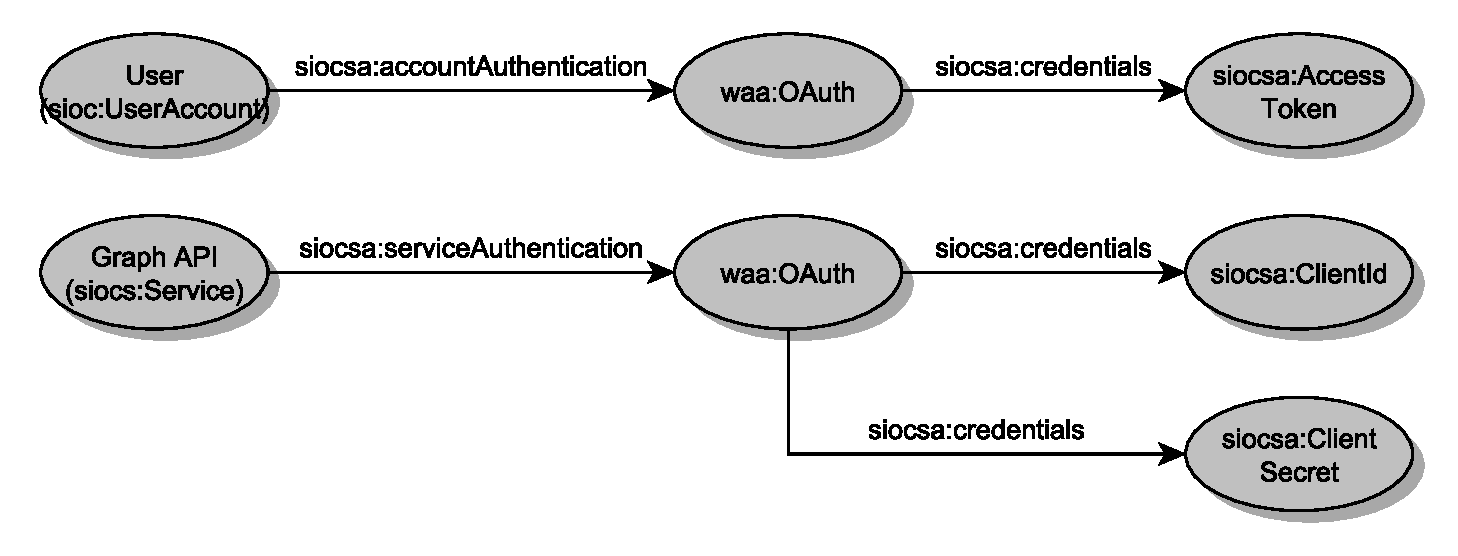
\includegraphics[
        width=\textwidth,
        keepaspectratio=true]
    {assets/images/mapping/facebook_useraccount_mapping}
    \caption{ Authentifizierungsdaten für Facebook in SIOC}
    \label{fig:facebook_useraccount_mapping}
\end{figure}

% subsubsection facebook_mapping_nach_sioc (end)

\subsubsection{Besonderheiten bei der Entwicklung des FacebookConnectors} % (fold)
\label{ssub:besonderheiten_bei_der_entwicklung_des_facebookconnectors}

Wie im Abschnitt über die Graph API schon beschrieben, ist es nahezu unmöglich an einer URI von Facebook zu erkennen, welcher Typ von Ressource sich dahinter befindet. Deshalb muss bei jeder unbekannten URI erst einmal alle Informationen mit dem Parameter \texttt{metadata=1} heruntergeladen geladen  und anhand der vorhanden Connections ermittelt werden, ob es sich um einen Beitrag, eine Wall oder etwas komplett anderes handelt. Deshalb ist es wichtig solche Erkenntnisse sofort in den Triplestore zwischenzuspeichern, um erneute Abfragen zu vermeiden.

% subsubsection besonderheiten_bei_der_entwicklung_des_facebookconnectors (end)

% subsection facebook_connector (end)

\subsection{GooglePlusConnector} % (fold)
\label{sub:google_plus_connector}

Der GooglePlusConnector ist die Implementierung eines Connectors für das soziale Online-Netzwerk Google+. Die Struktur ist der von Facebook in etwa gleich, wobei Google sie anders umgesetzt hat. Google+ verwendet, wie viele andere Plattformen auch, eine REST-basierte API mit JSON als Datenformat und OAuth zur Autorisierung der Abfragen. Leider ist zurzeit nur das Lesen von öffentlichen Beiträgen, aber kein Schreiben möglich. Trotzdem wurde für diese Plattform ein Connector implementiert, da gehofft wurde dass bis zum Ende dieser Arbeit die noch zum Schreiben fehlenden Operationen fertig sein würden. Was sich aber nicht bewahrheitet hatte.

% \begin{itemize}
%     \item Einfach REST API + JSON
%     \item OAuth
%     \begin{itemize}
%         \item Refreshtoken (token laufen quasi nie ab)
%         \item holen von token ohne webbrowser möglich
%     \end{itemize}
%     \item Objekte aufgebaut aus Actor (wer machte was), Verb(wie machte er es), Object (wtas machte er) + Metadata
%     \item verschieden Sprachen + Plattformen
%     \item lesen nur von öffentlichen Beiträgen
%     \item kein Schreiben von Beiträgen
% \end{itemize}

\subsubsection{Google+ API} % (fold)
\label{ssub:google_api}

Die API von Google für den Zugriff auf sein soziales Online-Netzwerk (siehe \cite{GooglePlusApi}) baut wie viele andere auch auf den REST-Prinzipien auf. Die URIs für die Anfragen beginnen mit \texttt{https://www.googleapis.com/plus/v1/} und danach folgt der Pfad zu den Ressourcen mit etwaigen Parameter. Die für hier wichtigsten Parameter sind \texttt{access\_token}, zum Angeben eines OAuth Accesstokens und dem Parameter \texttt{fields}, mit dem nur die dort angegebenen Datenfelder im Ergebnis zurückgeliefert werden. Als Datenformat wird JSON eingesetzt, aber mit einen von Facebook vollkommen unterschiedlichen Aufbau. Beiträge die als Activitys und Comments bezeichnet werden, bestehen im Grunde aus drei Teilen:

\begin{description}
    \item[\textbf{Actor:}] Der Actor-Eintrag sagt über die Ressource aus, von wem sie erstellt wurde. 
    \item[\textbf{Verb:}] Das Verb beschreibt auf welche Weise diese Ressource erstellt wurde. Für Activitys ist die Angabe von \enquote{post}, wenn ein Beitrag vom Actor selber geschrieben oder \enquote{share}, wenn dieser nur geteilt wurde und von jemand anderem stammt. 
    \item[\textbf{Object:}] Der Object-Eintrag enthält den eigentlichen Inhalt.
\end{description}

Neben diesen drei enthält eine Ressource noch Metadaten wie ID, Zeitpunkt der Veröffentlichung oder Änderung, Ortsdaten und andere mehr.

Die Google+ API teilt zu lange Ergebnislisten, ebenfalls wie Facebook, in mehrere Teillisten auf die wiederum auf einzelne Seiten aufgeteilt werden. Ob eine Seite der aktuellen folgt, kann über die Existenz des \texttt{nextPageToken} Eintrags erkannt werden. Dieser \emph{PageToken} muss für die Abfrage der nächsten Seite an die gleiche URI als Parameter \texttt{pageToken} angehängt werden. 

Wie schon erwähnt setzt die Google+ API für die Autorisierung auf OAuth 2.0. Ein Accesstoken ist aber nur nötig, wenn Operationen stellvertretend für einen Benutzer ausgeführt werden müssen. Für alle anderen Fälle ist ein API-Schlüssel vollkommen ausreichend. Zusätzlich zum Accesstoken liefert Google+ auch einen Refreshtoken mit. So können abgelaufene Accesstoken vom Programm automatisch wieder reaktiviert werden, ohne dass der Benutzer dies von Hand machen muss. Die für die Erstellung von Access- und Refreshtoken gebrauchten Client-ID und Client-Secret werden über die \emph{Google API Console}\footnote{\url{https://code.google.com/apis/console}} erstellt. Wichtig dabei ist eine \enquote{Client ID for installed applications} auszuwählen. Sowohl für den Zugriff auf die REST-API, als auch für die Erstellung der Token, stellt Google eine Java-Bibliothek zur Verfügung. 

\begin{lstlisting}[
    caption={Google+ API Java: Access- und Refreshtoken}\label{lst:gplus_java_accesstoken},
    captionpos=t]
GoogleAuthorizationCodeFlow flow = new GoogleAuthorizationCodeFlow.Builder(
        new NetHttpTransport(),
        new JacksonFactory(),
        CLIENT_ID,
        CLIENT_SECRET,
        Arrays.asList("https://www.googleapis.com/auth/plus.login"))
    .build();

Credential credentials = new AuthorizationCodeInstalledApp(
        flow,
        new LocalServerReceiver())
    .authorize("user");
\end{lstlisting}

Listing \ref{lst:gplus_java_accesstoken} zeigt wie man sich Access- und Refreshtoken für Google+ in Java holen kann. Von Zeile Eins bis 9 wir ein sogenannter \enquote{AuthorizationCodeFlow} erzeugt. Dieser abstrahiert für das Programm den OAuth-Mechanismus, über den man die Token von Google bezieht. In der Zeile 2 und 3 bekommt dieser CodeFlow externe Objekte übergeben mit dem er HTTP-Operationen ausführen und die zurückgelieferten Daten verarbeiten kann. In den zwei Folgezeilen werden die Client-ID und das Client-Secret übergeben. In der sechsten Zeile muss, wie schon bei Facebook, ein Geltungsbereich (Scope) für den Accesstoken festgelegt werden. In diesem Falle wollen wir mit \enquote{\texttt{https://www.googleapis.com/auth/plus.login}} Operationen stellvertretend für einen Benutzer ausführen. In Zeile 8 wird das Code-Flow-Objekt über die \texttt{build()}-Methode erzeugt. Für Desktopprogramme wird wieder eine externer Internetbrowser zum Holen der Token benötigt. Doch auch dafür bietet Google eine fertige Klasse an, die (fast) alle Schritte automatisiert. Diese Klasse heißt \texttt{AuthorizationCodeInstalledApp}. Ihr werden der obige CodeFlow und ein lokaler Webserver (ebenfalls schon fertig vorhanden) übergeben und über die Methode \texttt{authorize(\dots)} die Token erzeugt. Die Zeichenkette \enquote{\texttt{user}} ist nur von Bedeutung, wenn man dem CodeFlow noch einen \enquote{DataStore} für die Accestoken mit gibt, was hier weggelassen wurde. Im Anhang \ref{sec:oauthtool} ist die kurze Beschreibung eines Hilfsprogramms zum Erstellen von Accesstokens für Google+ zu finden.

\begin{lstlisting}[
    caption={Google+ API: Zugriff auf Activity-Feed mit Java}\label{lst:gplus_activity_feed_java},
    captionpos=t]
Plus plus = new Plus.Builder(
        new NetHttpTransport(), 
        new JacksonFactory(),
        credential)
    .setApplicationName(APPLICATION_NAME)
    .build();

ActivityFeed activityFeed = plus.activities()
    .list( "me","public" )
    .execute();

for(Activity activity : activityFeed.getItems()){
    System.out.println(
        activity.getActor().getDisplayName() 
        + ": " 
        + activity.getObject().getContent());
}
\end{lstlisting}

Das kleine Beispiel in Listing \ref{lst:gplus_activity_feed_java} zeigt wie auf einen Activity-Feed, also die Liste der geschriebenen Beiträge eines Benutzers, in Google+ mit Java zugegriffen werden kann. Von Zeile Eins bis 6 wird der Client für den Zugriff auf Google+ mit einen Builder\footnote{\enquote{Builder}-Entwurfsmuster: \url{http://www.oodesign.com/builder-pattern.html}} gebaut. Als Argument wird wieder das Objekt einer Klasse für die Verwendung von HTTP-Operationen und eines für das Arbeiten mit JSON übergeben. Als dritter Parameter in Zeile 4 kommen noch die Credentials aus Listing \ref{lst:gplus_java_accesstoken} mit dazu. Mit der Methode \texttt{setApplicationName(\dots)} kann noch ein Name für die Anwendung angegeben werden bevor der Client mit der Methode \texttt{build()} in Zeile 6 erstellt wird. Der Client enthält mehrere Methoden mit denen man auf die verschiedenen Ressource wie Activitys, Kommentare und Personen zugreifen kann. In Zeile 8 wird die Methode \texttt{activities()} eingesetzt, um an eine Hilfsklasse für alle Activitys zu gelangen, welche die Operationen zum Lesen eines Activity-Feeds, nur eines einzelnen Activitys oder der Suche nach anderen Activitys enthält. Mit \texttt{list("me", "public")} wird eine Abfrage für den \enquote{public} Activity-Feed (nur dieser ist aktuell verfügbar) des Benutzers mit der ID \enquote{me} (Steht immer für den aktuell angemeldeten Benutzer) erstellt, die dann mit dem Aufruf der Methode \texttt{execute()} des zurückgelieferten Objekts ausgeführt wird. Das Ergebnis dieser Abfrage enthält ein Array von Activitys, das von der Methode \texttt{getItems()} zurückgegeben wird. Zum Schluss werden von allen Activitys der Name des Autors und der Inhalt ausgegeben. Ist ein oben erwähnter Pagetoken für eine weiter Ergebnisseite vorhanden, kann dieser an das Objekt, was von \texttt{list("me", "public")} zurückgegeben wird, mit der Methode \texttt{setPageToken(\dots)} übergeben werden bevor \texttt{execute()} ausgeführt wird.

% subsubsection google_api (end)

\subsubsection{Mapping von Google+ nach SIOC} % (fold)
\label{ssub:google_mapping_nach_sioc}

Die Struktur in Google+ ist annähernd mit der von Facebook gleich. Jeder Benutzer hat seinen eigenen ActivityFeed auf dem er Beiträge in der Form von Activitys veröffentlichen kann. Demzufolge entspricht ein ActivityFeed der SIOC-Klasse \texttt{sioc:Forum}, wobei dieser die Activitys als \texttt{sioc:Post} enthält. Kommentare auf Activitiys werden ebenfalls \texttt{sioc:Post} zugeordnet, wobei sie sich immer genau auf ein Activity beziehen und niemals auf ein anderen Kommentar (Siehe Abbildung \ref{fig:googleplus_sioc_mapping}). 

\begin{minipage}{\textwidth}
    \centering
    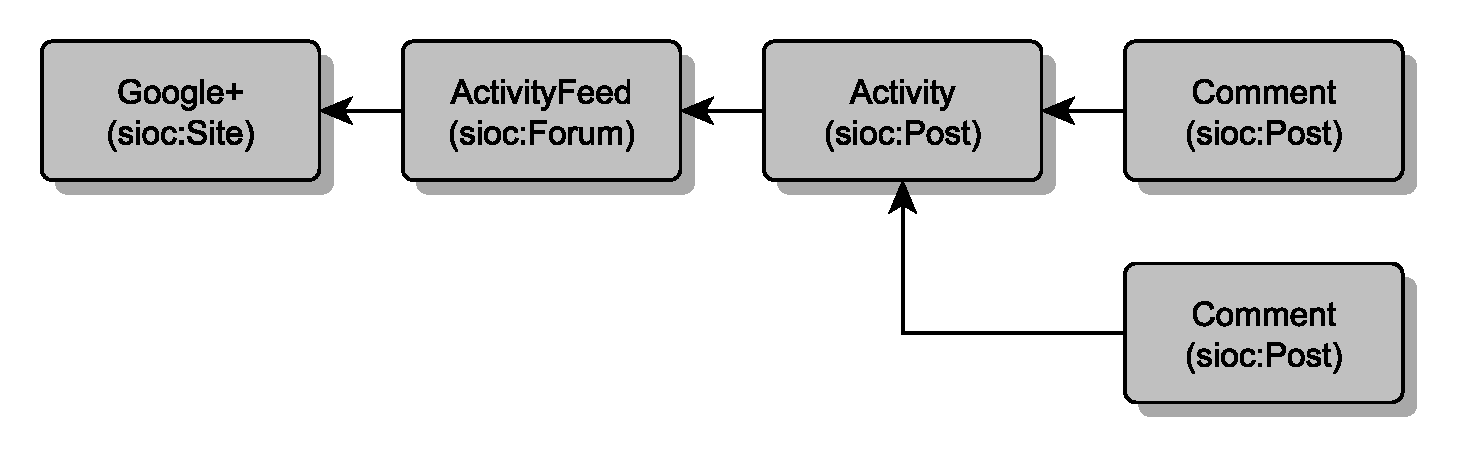
\includegraphics[
        width=0.8\textwidth,
        keepaspectratio=true]
    {assets/images/mapping/googleplus_sioc_mapping}
    \captionof{figure}{Struktur von Google+ und Mapping nach SIOC}
    \label{fig:googleplus_sioc_mapping}
\end{minipage}

Wie schon Facebook setzt Google+ auf OAuth 2.0 für die Google+ API. Jedoch verwendet Google+ für den Client noch einen zusätzlichen Refreshtoken, um die Accesstoken automatisch aktualisieren zu können, falls diese abgelaufen sind (Siehe Abbildung \ref{fig:googleplus_useraccount_mapping}). Bei der Servicebeschreibung muss wieder die Client-ID und das Client-Secret als Credentials einem Objekt der Klasse \texttt{waa:OAuth} mit der Eigenschaft \texttt{siocsa:serviceAuthentication} mitgegeben werden.

\begin{minipage}{\textwidth}
    \centering
    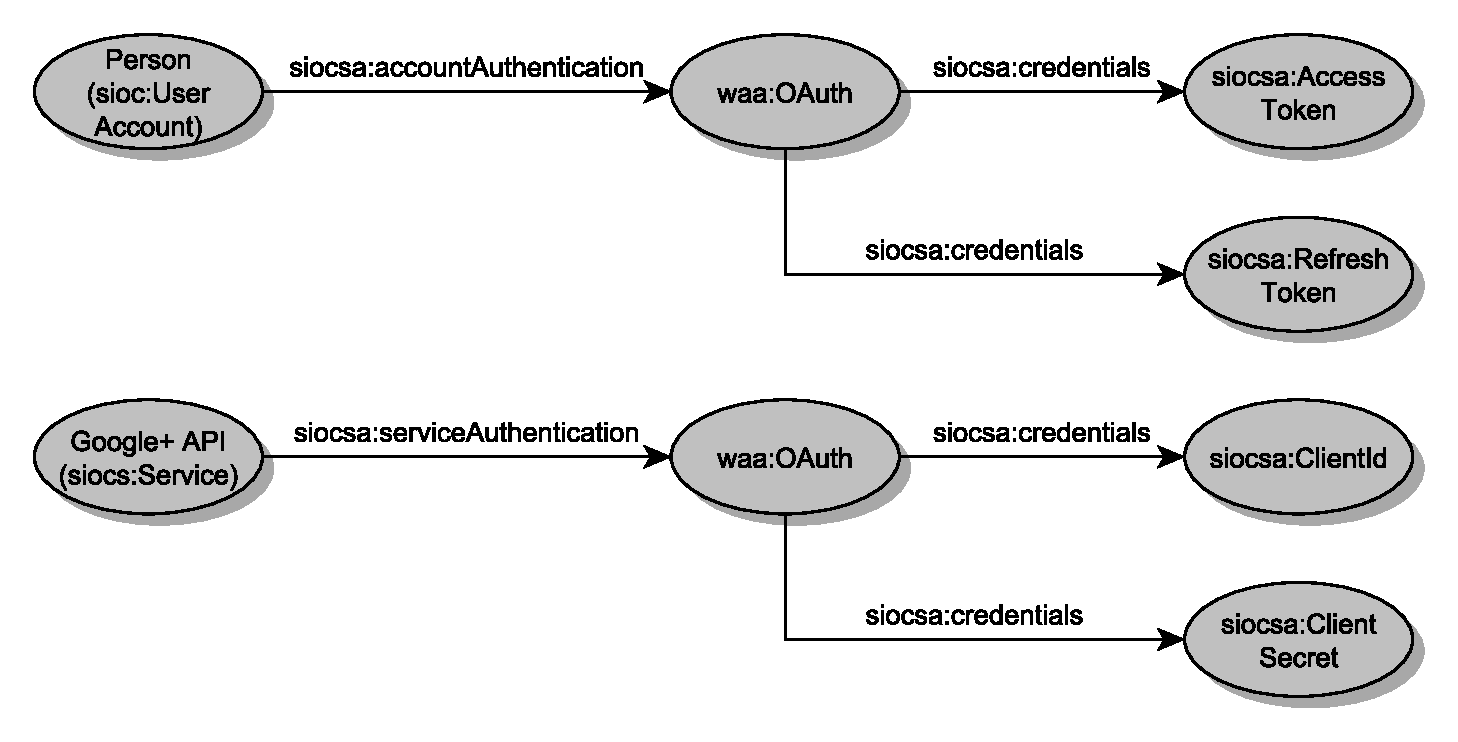
\includegraphics[
        width=\textwidth,
        keepaspectratio=true]
    {assets/images/mapping/googleplus_useraccount_mapping}
    \captionof{figure}{ Authentifizierungsdaten für Google+ in SIOC}
    \label{fig:googleplus_useraccount_mapping}
\end{minipage}

In Tabelle \ref{tbl:googleplus_rdf_uri_format} stehenden URIs für die Google+ Ressourcen in RDF entsprechen selbigen wie für die REST-Abfragen. Die einzige Einschränkung ist, dass in der aktuellen Version der Google+ API bei der URI für den ActivityFeed (\texttt{sioc:Forum}) für den Platzhalter \enquote{\texttt{\{collection\}}} nur der Wert \enquote{public} zulässig ist.

\begin{table}[ht]
    \centering
    \caption{Format der URIs für Google+ in RDF}
    \begin{tabular}{l|p{13cm}}
        \textbf{SIOC Klasse} & \textbf{URI-Format}\\ 
        \hline
        \texttt{sioc:Site} & 
        \texttt{http://plus.google.com/} \\

        \texttt{sioc:Service} & 
        \texttt{https://www.googleapis.com/plus/v1} \\

        \texttt{sioc:UserAccount} & 
        \texttt{https://www.googleapis.com/plus/v1/people/\{userId\}} \\

        \texttt{sioc:Forum} & 
        \texttt{\{userAccountUri\}/activities/\{collection\}} \\

        \texttt{sioc:Thread} & 
        \texttt{https://www.googleapis.com/plus/v1/activities/\{activityId\}} \\

        \texttt{sioc:Post} & 
        \texttt{https://www.googleapis.com/plus/v1/comments/\{commentId\}} \\
    \end{tabular}
    \label{tbl:googleplus_rdf_uri_format}
\end{table}

% subsubsection google_mapping_nach_sioc (end)

% subsection google_plus_connector (end)

\subsection{YoutubeConnector} % (fold)
\label{sub:youtube_connector}

Der YoutubeConnector ist der letzte Connector, das als Demonstration für SOCC implementiert wurde. Google ist zum Zeitpunkt an dem diese Arbeit geschrieben wurde dabei seine API und Youtube allgemein umzubauen. Da die neue API noch nicht 100\% alle Funktionen unterstützt, musste eine älter Version eingesetzt werden. Die Verwendung der API und das Mapping nach SIOC gingen aber ohne große Probleme.


% \begin{itemize}
%     \item Aktueller Umbau der API (ähnlich google+) v3
%     \begin{itemize}
%         \item keine lesen von kommentaren
%         \item kein schreiben
%     \end{itemize}
%     \item alte GData Feed API v2 basiert auf RSS + Youtube Erweiterung
%     \item Mapping teilweise durch basis auf RSS einfach, manchmal auch nicht
%     \item Wichtigen Metadaten nur implizit vorhanden (comment id in uri aber nicht in datenformat)
% \end{itemize}

\subsubsection{Youtube Data API} % (fold)
\label{ssub:youtube_data_api}

Für Youtube existieren zurzeit zwei verschiedene APIs, eine Version 3 und die ältere Version 2. \emph{Die Youtube Data API \textbf{v3}} befindet sich noch im Entwicklungsstadium. Dort ist es zum Beispiel noch nicht möglich Kommentare von Video zu lesen, geschweige denn zu schreiben. Aus diesem Grund muss für den YoutubeConnector die älter \emph{Youtube Data API \textbf{v2}} benutzt werden, welche diese Funktionen noch bietet. 

Die Youtube Data API v2 baut auf dem \emph{Google Data Protokoll} auf. Eine API nach dem REST-Prinzip mit Atom und JSON als Datenformat. Für Youtube wird aber primär Atom eingesetzt (umschalten auf JSON ist möglich). Die einzelnen Ressourcen können als Atom-Feed, also eine Liste einzelnen Einträgen wie die einer Playliste, oder als ein einzelnes Entry-Element, zum Beispiel Informationen zu einen Benutzerkonto, zurückgegeben werden. Youtube verwendet aber nicht nur die vom Atom-Standard definierten Elemente, sondern ergänzt das Format durch eine große Zahl eigener Erweiterungen wie Spieldauer eines Videos, Statistiken, Bewertungen oder Informationen zu Benutzerkonten. Jeder Feed/Eintrag enthält mehrere Link-Element die auf weiterführenden Ressourcen verweisen. Ist die Menge der Einträge eines Feedes zu groß, wird das Ergebnis auf mehrere Feeds aufgeteilt. Um zwischen diesen Teilergebnissen zu navigieren, enthalten die Teilfeeds Links auf ihren Vorgänger- und/oder Nachfolge-Feeds (siehe Listing \ref{lst:ytdataapi_navigation_through_results}).

\begin{lstlisting}[
    language=XML,
    caption={Youtube Data API v2: Navigation durch die Ergebnisse}\label{lst:ytdataapi_navigation_through_results},
    captionpos=t]
<link rel='previous' type='application/atom+xml'
  href='http://gdata.youtube.com/feeds/api/videos?start-index=1&max-results=25...'/>
<link rel='next' type='application/atom+xml'
  href='http://gdata.youtube.com/feeds/api/videos?start-index=51&max-results=25...'/>
\end{lstlisting}

Alle Ressourcen auf die öffentlich zugegriffen werden kann, brauchen keine vorherige Anmeldung. Sollen aber zum Beispiel Kommentare geschrieben werden, ist eine Anmeldung notwendig. Für der Programm muss ein ein API-Schlüssel (von Google \enquote{Developer Key} genannt) im \emph{Product Dashboard}\footnote{\url{http://code.google.com/apis/youtube/dashboard/}} erstellt werden. Dieser API-Schlüssel wird dann jeder Anfrage als URI Parameter \texttt{key={apiKey}} angehängt. Soll auch stellvertretend für einen Benutzer Kommentare geschrieben werden, ist noch zusätzlich der Benutzername und das Password von ihm Voraussetzung.

Google bietet selber eine Java API für die Youtube Data API v2 an, mit der das Auslesen, Verarbeiten und Senden der Atom Feeds und Einträge sehr einfach ist. Das Programmbeispiel in Listing \ref{lst:ytdataapi_youtube_service} zeigt eine Beispiel für die Verwendung der Youtube Data API in Java. Ausgangspunkt in Zeile Eins ist die Klasse \texttt{YouTubeService} die als Client eingesetzt wird. Bei der Erzeugung eines Objektes dieser Klasse wird eine beliebige Zeichenkette als Client-ID (nicht zu verwechseln mit der Client-ID von OAuth 2.0) und der oben beschriebene API-Schlüssel benötigt. In der zweiten Zeile werden der Benutzername und das Password an den Client übergeben. Für das Auslesen eines Atom-Feeds wird die Methode \texttt{getFeed(\dots)} eingesetzt. Ihr werden in Zeile 5 die URI zum gesuchten Feed und in Zeile 6 die Klasse in die der Feed aus dem XML-Format konvertiert werden soll übergeben. In diesen Fall steckt hinter der URI eine Playliste mit mehreren Videoeinträgen. In Zeile 8 bis 11 werden dann die Titel und der Link auf das Video ausgegeben.

\begin{lstlisting}[
    caption={Youtube Data API v2: Java YouTubeService}\label{lst:ytdataapi_youtube_service},
    captionpos=t]
YouTubeService service = new YouTubeService(clientId, apiKey);
service.setUserCredentials(username, password);

VideoFeed videoFeed = service.getFeed(
    new URL("http://gdata.youtube.com/feeds/api/playlists/PL59AFCB0F92BB89A9"), 
    VideoFeed.class);

for(VideoEntry videoEntry : videoFeed.getEntries() ) {
    System.out.println(videoEntry.getTitle() 
        + ": " 
        + videoEntry.getSelfLink());
}
\end{lstlisting}

Wurde das Ergebnis in mehrere Teilfeeds aufgeteilt, dann ist der Rückgabewert der Funktion \texttt{videoFeed.getNextLink()} ungleich \texttt{null}. Ist dies der Fall kann der nächste Teilfeed wieder mit der Methode \texttt{service.getFeed(\dots)} und der URI des von \texttt{getNextLink()} zurückgegebenen Links geholt werden.

\begin{lstlisting}[
    caption={Youtube Data API v2: Kommentar schreiben}\label{lst:ytdataapi_kommentar_schreiben},
    captionpos=t]
commentUrl = "http://gdata.youtube.com/feeds/api/videos/oHg5SJYRHA0/comments";
CommentEntry newComment = new CommentEntry();
newComment.setContent(new PlainTextConstruct("Tolles Video!! :)"));
service.insert(new URL(commentUrl), newComment);
\end{lstlisting}

Das Schreiben eines Eintrags ist in Listing \ref{lst:ytdataapi_kommentar_schreiben} dargestellt. Die URI zum Schreiben in Zeile Eins zeigt auf einen Kommentar-Feed für das Video mit der ID \enquote{oHg5SJYRHA0}. In der zweiten Zeile wird dann zunächst eine Objekt der Klasse \texttt{CommentEntry} erstellt und in Zeile 3 mit dem Inhalt der Nachricht befüllt. Dieses Objekt wird dann zusammen mit der URI aus Zeile Eins der Methode \texttt{insert(\dots)} übergeben. Für diese Methode ist das vorherige übergeben von Benutzername und Passwort Pflicht, da sonst Youtube mit einen Fehler antwortet.

\subsubsection{Mapping von Youtube nach SIOC} % (fold)
\label{ssub:youtube_mapping_nach_sioc}

Der Aufbau von Youtube unterscheidet sich etwas von den anderen vier Plattformen, da es vorrangig zum Austausch von Videos gedacht ist. Nichtsdestotrotz ist es möglich in den Kommentaren über diese Videos zu diskutieren. Videos können dabei an zwei unterschiedlichen Orten liegen. Entweder sind sie unter den hochgeladenen Videos eines Benutzers zu finden oder in einer von ihm angelegen Playliste. Sowohl die Liste der hochgeladenen Videos (Uploads) als auch die Menge angelegter Playlisten (Playlists) können der SIOC-Klasse \texttt{sioc:Forum} zugeordnet werden. Eine Playliste enthält in der Regel Videos mit einem thematischen Schwerpunkt, wie zum Beispiel Musik Genre, Rezepte, Katzenvideos und so weiter. Dies ist den Threads in einen Forum sehr ähnlich, wodurch \texttt{sioc:Thread} für eine Playliste die beste Wahl für das Mapping nach SIOC ist. Die in den Uploads und Playlisten enthaltenen Videos entsprechen den Startbeitrag einer Diskussion, die den Inhalt des Videos als Thema hat. Eine Zuordnung von Videos zu \texttt{sioc:Post} ist daher naheliegend. Das Video wird dann als \texttt{sioc:attachment} an diesen \texttt{sioc:Post} angehängt. Videos können seit September 2013 nicht mehr eine Antwort auf ein anderes Video sein (siehe \cite{YTCreators2013}), somit sind Kommentare die einzigen Beiträge, die mit einem Video verbunden sind. Die genauen Beziehungen sind noch einmal in Abbildung \ref{fig:youtube_sioc_mapping} zu sehen.

\begin{figure}[ht]
    \centering
    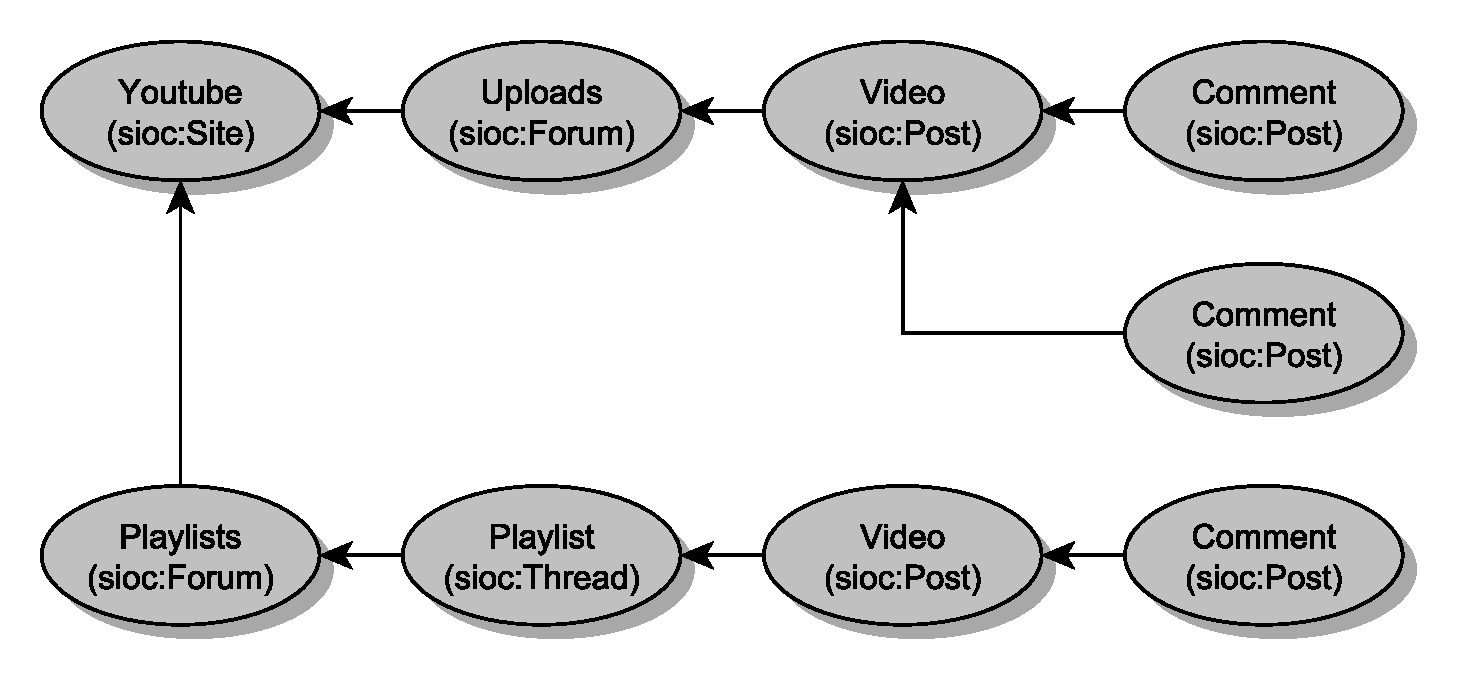
\includegraphics[
        width=0.8\textwidth,
        keepaspectratio=true]
    {assets/images/mapping/youtube_sioc_mapping}
    \caption{Struktur von Youtube und Mapping nach SIOC}
    \label{fig:youtube_sioc_mapping}
\end{figure}

Der Zugriff auf die Funktionen der Youtube Data API, die Daten verändern können, wird nur gewährt, wenn der Benutzername und das Password eines Benutzers angegeben werden. Die Angabe erfolgt schon wie bei Moodle über die Klasse \texttt{waa:Direct} mit der Eigenschaft \texttt{siocsa:accountAuthentication} für den betreffenden \texttt{sioc:UserAccount}. Zusätzlich muss der API-Schlüssel, der für das Programm erstellt wurde, der Servicebeschreibung \texttt{sioc:Service} hinzugefügt werden. Dies gelingt über die Eigenschaft \texttt{siocsa:serviceAuthentication} mit der Klasse \texttt{waa:WebAPI} und dem API-Schlüssel als Credential mit der Klasse \texttt{waa:APIKey}.

\begin{figure}[!ht]
    \centering
    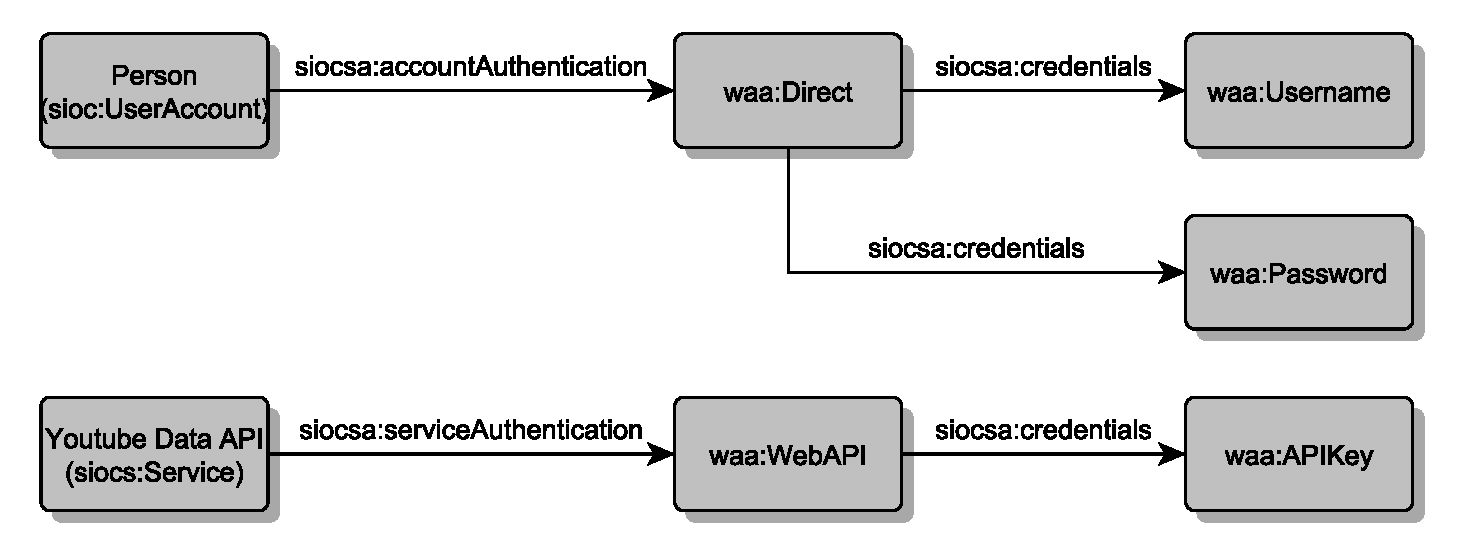
\includegraphics[
        width=0.87\textwidth,
        keepaspectratio=true]
    {assets/images/mapping/youtube_useraccount_mapping}
    \caption{ Authentifizierungsdaten für Youtube in SIOC}
    \label{fig:youtube_sioc_mapping_useraccount_mapping}
\end{figure}

Für die RDF-URIs der Youtube Ressourcen wurden die gleichen wie für den Zugriff auf die Youtube Data API verwendet (Siehe Tabelle \ref{tbl:youtube_rdf_uri_format}. Die URIs bauen teilweise wieder aufeinander auf, so dass ein Teil der Struktur in der sie sich befinden rekonstruiert werden kann. Zum Beispiel baut die URI für ein Kommentar auf der für ein Video auf. So erkennt man sofort zu welchen Video der Kommentar gehört, ohne die Daten des Kommentars herunterzuladen zu müssen. 

\begin{table}[ht]
    \centering
    \caption{Format der URIs für Youtube in RDF}
    \begin{tabular}{l|p{13cm}}
        \textbf{SIOC Klasse} & \textbf{URI-Format}\\ 
        \hline
        \texttt{sioc:Site} & 
        \texttt{http://www.youtube.com/} \\

        \texttt{sioc:Service} & 
        \texttt{http://gdata.youtube.com} \\

        \texttt{sioc:UserAccount} & 
        \texttt{http://gdata.youtube.com/feeds/api/users/\{userId\}} \\

        \texttt{sioc:Forum} & 
        \texttt{\{userAccountUri\}/uploads} \emph{oder} \newline \texttt{\{userAccountUri\}/playlists} \\

        \texttt{sioc:Thread} & 
        \texttt{http://gdata.youtube.com/feeds/api/playlists/\{playlistId\}} \\

        \texttt{sioc:Post} & 
        \texttt{http://gdata.youtube.com/feeds/api/videos/\{videoId\}} \emph{oder} \newline \texttt{http://gdata.youtube.com/feeds/api/videos/\{videoId\} \newline /comments/\{commentId\}} \\
    \end{tabular}
    \label{tbl:youtube_rdf_uri_format}
\end{table}


% subsubsection youtube_mapping_nach_sioc (end)

\subsubsection{Besonderheiten bei der Implementierungs des YoutubeConnectors} % (fold)
\label{ssub:besonderheiten_bei_der_implementierungs_des_youtubeconnectors}

Vorteil der Youtube Data API v2 ist die Verwendung von Atom als Datenformat. So sind schon viele URIs auf weiterführende Ressourcen vorhanden. Leider wird eine Anwendung sehr schnell von Youtube blockiert, wenn diese zu oft hintereinander Abfragen sendet. Aus diesem Grund muss zwischen zwei Abfragen immer eine bestimmte Zeit vergangen sein, bevor die nächste abgeschickt werden kann. Am Besten hat sich eine Zeitspanne von 500\,ms bewährt, welche aber ab und zu immer noch Probleme macht. Diesen Wert aber höher zu stellen verlangsamt das komplette System, da manchmal mehrere Abfragen gemacht werden müssen, bis alle gesuchten Informationen vorhanden sind. Zusätzlich sind nicht alle Informationen explizit über die Java-API zugänglich. Zum Beispiel erhält die Klasse für Kommentare keine Methode für den Zugriff auf die Video und Kommentar-ID. Diese muss aus der URI des Kommentars erste extrahiert werden.

% subsubsection besonderheiten_bei_der_implementierungs_des_youtubeconnectors (end)

% subsubsection youtube_data_api (end)

% subsection youtube_connector (end)

% section implementierung_einiger_connectoren (end)

\section{Implementierung von SOCC-Camel} % (fold)
\label{sec:implementierung_von_socc_camel}

Die Implementierung des SOCC-Camel Moduls als Komponente für Camel ist relativ unkompliziert. Die Java-API von Camel enthält schon viele vorbereitet Klassen, von denen die Klassen für SOCC-Camel abgeleitet werden können. Danach ist nur noch wenig Arbeit zusätzlich zu machen.

\begin{description}
    \item[\textbf{SoccComponent:}] Die Klasse SoccComponent muss die in der Konfigurations-URI angegeben Connectoren mit den Daten aus den Triplestore erzeugen, verwalten und für jeden Endpunkt eine Objekt der Klasse SoccEndpoint mit dem Parametern und dem Connector erzeugen. 

    \item[\textbf{SoccEndpoint:}] Die Klasse SoccEndpoint ist wiederum nur eine Fabrik für den SoccPostPollConsumer und den SoccPostProducer. 

    \item[\textbf{SoccPostPollConsumer:}] Die komplette Arbeit des SoccPostPollConsumer findet in der Methode \texttt{poll()} statt, die aus der abgeleiteten Klasse ScheduledPollConsumer von Camel überschrieben wird. Das Listing \ref{lst:socc_camel_polling_code} zeigt den Quellecode dieser Methode. In der zweiten Zeile wird der PostReader des Connectors aufgerufen, wobei die Variable \texttt{lastPollTime} den Zeitpunkt enthält, an dem \texttt{poll()} das letzte mal aufgerufen wurde. Ist mindesten ein Beitrag in der zurückgelieferten Liste, werden diese ab Zeile 4 serialisiert, in eine Nachricht verpackt und an Camel zum Versenden übergeben. Mit RDF2Go können leider nur komplette Triplestores serialisiert werden, deswegen müssen die Daten der Beiträge erst in einen neuen, leeren Triplestore kopiert werden, so dass nicht auch unerwünschte Daten mitgeschickt werden die noch im Triplestore des Connectors liegen. Dieser temporäre Triplestore wird in Zeile 5 und 6 angelegt. Der Quellcode in den Zeilen 9 bis 13 kopiert erst alle Prefixe aus dem originalen Triplestore in den neuen. Dieser Schritt ist zwar nicht zwingend notwendig, erleichtert aber das lesen der serialisierten RDF-Daten für das Debuggen. In den Zeilen 15 bis 20 werden dann alle RDF-Daten der Beiträge in das temporäre Model kopiert. Danach kann ab Zeile 22 angefangen werden die zu sendende Nachricht zusammen zu bauen. Die serialisierten Daten kommen dann in Zeile 23 als \enquote{Body} in die Nachricht. Zusätzlich wird in Zeile 27 das verwendete Serialisierungsformat als MIME-Type angegeben. Nachrichten werden in Camel zusätzlich in eine Art Umschlagt der Klasse \texttt{Exchange} verpackt. Das verwenden der Methode \texttt{setIn(\dots)} sagt dabei Camel, dass diese Nachricht als eingehende Nachricht für einen anderen Endpunkt gedacht ist. Möchte man auf eine Nachricht eine Antwort schicken, macht man dies mit der Methode \texttt{setOut(\dots)}. In Zeile 33 wird die Nachricht dann abgeschickt. Am Ende muss dann nur noch die Variable \texttt{lastPollTime} auf die aktuell Zeit aktualisiert werden.
 
\begin{lstlisting}[
caption={Quellcode zum Polling im  SoccPostPollConsumer}\label{lst:socc_camel_polling_code},
captionpos=t]
protected int poll() throws Exception {
    List<Post> posts = postReader.pollPosts(uri, lastPollTime, limit);
    if ( !posts.isEmpty() ) {
        Model tmpModel = RDF2Go.getModelFactory().createModel();
        tmpModel.open();

        try {
            Model model = postReader.getConnector().getContext()
            .getModel();
            for (Entry<String, String> entry : model.getNamespaces().entrySet()) {
            tmpModel.setNamespace(entry.getKey(), entry.getValue());
            }

            for (Post post : posts) {
                tmpModel.addAll( 
                    RdfUtils.getAllStatements( 
                        model, 
                        post ).iterator() );
            }

            Message msg = new DefaultMessage();
            msg.setBody( 
                RdfUtils.modelToString(
                    tmpModel, 
                    Syntax.RdfXml));
            msg.setHeader(
                Exchange.CONTENT_TYPE, 
                Syntax.RdfXml.getMimeType());

            Exchange ex = getEndpoint().createExchange();
            ex.setIn(msg);
            getProcessor().process(ex);
        } finally {
            tmpModel.close();
        }
    }

    lastPollTime.setTime( System.currentTimeMillis() );
}
\end{lstlisting}

    \item[\textbf{SoccPostProducer:}] Die Klasse SoccPostProducer ist wieder nur sehr unspektakulär. Sie nimmt alle ankommenden Nachrichten, holt die serialisierten Daten aus dem Body, überprüft ob ein gültiger MIME-Type vorliegt und gibt alles an den PostWriter des Connectors weiter. 
    
\end{description}

%\todo[inline]{Text schreiben}

% section implementierung_von_socc_camel (end)

\section{Proof of Concept} % (fold)
\label{sec:proof_of_concept}

Um die Funktionsweise von SOCC und SOCC-Camel zu demonstrieren, soll nun ein \enquote{Proof of Concept} erstellt werden. Hierzu wird ein Programm vorgestellt, das die Beiträge einer Diskussion aus Canvas mit den Kommentaren eines Beitrags aus einer Facebook-Gruppe synchronisiert. Danach wird die Ausführung dieses Programm Schritt für Schritt erklärt und gezeigt welche Daten ausgetauscht werden. In der Realität sind die gezeigten SIOC-Daten im RDF/XML-Format oder im Triplestore, aber aufgrund der besseren Lesbarkeit sind sie hier in Turtle dargestellt.

\subsection{Vorbereitungen} % (fold)
\label{sub:vorbereitungen}

Die Konfigurationsdaten für dieses Programm sind im Anhang \ref{sec:anhang_proof_of_concept_konfigurationsdaten} im Turtle-Format zu sehen. Dort befindet sich die Definitionen von den zwei Personen \enquote{Max Hiwi} und \enquote{Florian} mit jeweils ihren Benutzerkonten für Canvas und Facebook. Für beide Plattformen wurde für die Benutzerkonten Accesstoken erstellt und dort hinterlegt. Beide Personen erlauben einen öffentlichen Zugriff auf all ihre Beiträge durch eine ACL-Autorisierung. Ebenfalls wurden die Servicebeschreibungen und die Konfigurationen für die Canvas und Facebook Connectoren angegeben. Der Service für Facebook enthält zusätzlich die Client-ID und den Client-Secret, um aus kurzlebigen Accesstoken welche mit einer Haltbarkeit von zwei Monaten generieren zu können, falls sie das nicht schon sind. Sowohl Accesstoken als auch Client-ID und Client-Secret wurden aus Datenschutzgründen nicht vollständig angeben.

Die Synchronisation zwischen Canvas und Facebook mit Camel soll dabei auf zwei Arten demonstriert werden. Der Nachrichtenweg von Canvas aus wird erst an ein JMS-Topic geschickt, bevor die Beiträge an den FacebookConnector weitergeben werden. Der umgekehrte Weg von Facebook nach Canvas erfolgt direkt durch Camel, ohne eine Verwendung von JMS. Als JMS-Provider wird das freie ActiveMQ von Apache eingesetzt. Dieser kann sowohl als eigener Server als auch eingebettet in einem Programm ausgeführt werden.

Zuerst muss für die Verwendung von ActiveMQ und SOCC der CamelContext mit den entsprechenden Komponenten vorbereitet werden. In Zeile Eins des Listings \ref{lst:poc_prepare_camel} wird ein Objekt dieses CamelContextes aus der Klasse \texttt{DefaultCamelContext} erzeugt. Um ActiveMQ von Camel aus nutzen zu können, muss ein Objekt der Klasse \texttt{ActiveMQComponent}\footnote{\url{http://camel.apache.org/activemq.html}} in Zeile 2 vorzugsweise unter dem Namen \enquote{activemq} registriert und die Adresse zum ActiveMQ Server angegeben werden. Danach folgt in Zeile 5 die Registrierung von SOCC-Camel mit dem Namen \enquote{socc}. Übergeben wird das Objekt des CamelContextes und ein SoccContext mit einem RDF2Go Model, in das zuvor die Konfigurationsdaten geladen wurden.  

\begin{lstlisting}[
    caption={Proof of Concept: CamelContext vorbereiten} \label{lst:poc_prepare_camel},
    captionpos=t]
DefaultCamelContext camelContext = new DefaultCamelContext();
camelContext.addComponent(
        "activemq",
        ActiveMQComponent.activeMQComponent( "tcp://localhost:61616" ) );
camelContext.addComponent(
        "socc",
        new SoccComponent( camelContext, new SoccContext( model ) ) );
\end{lstlisting}

Neben den in Abschnitt \ref{ssub:apache_camel} beschrieben Methode mit der Klasse \texttt{RouteDefinition}, können Routen auch mit der Klasse \texttt{RouteBilder} erstellt werden. Wie in Listing\ref{lst:poc_prepare_camel_routes} zu sehen. Die erste Route in Zeile 4 ist die von der Diskussion aus Canvas in das JMS-Topic mit der Bezeichnung \enquote{canvas-topic}. Die URI für den Start-Endpunkt enthält die ID des konfigurierten CanvasConnectors \enquote{poc-canvas}, der URI zur Diskussion \texttt{https://[\dots]/api/v1/courses/798152/discussion\_topics/1540697} und soll dieses alle fünf Minuten (300000 Millisekunden) nach neuen Beiträgen abfragen. Die zweite Route in Zeile 9 beschreibt den Weg aus dem JMS-Topic \enquote{canvas-topic} in den Connector mit der ID \enquote{poc-facebook}, der dann die Beiträge als Kommentare in den Beitrag hinter der URI \texttt{https://graph.facebook.com/520312298060793\_520417398050283} schreibt. Die letzte Route in Zeile 13 definiert den umgekehrten Weg, wobei der FacebookConnector ebenfalls alle fünf Minuten nach neuen Beiträgen schauen soll. Der eben erstellte RouteBuilder muss jetzt noch in Zeile 21 an den CamelContext übergeben und in Zeile 22 Camel gestartet werden.  

\begin{lstlisting}[
    caption={Proof of Concept: Routen vorbereiten} \label{lst:poc_prepare_camel_routes},
    captionpos=t]
RouteBuilder routeBuilder = new RouteBuilder() {
    @Override
    public void configure() throws Exception {
        from("socc://poc-canvas?uri=https://canvas.instructure.com/api/v1/"
            + "courses/798152/discussion_topics/1540697"
            + "&delay=300000" )
            .to("activemq:topic:canvas-topic");

        from( "activemq:topic:canvas-topic" )
            .to("socc://poc-facebook?uri=https://graph.facebook.com/"
                + "520312298060793_520417398050283");

        from("socc://poc-facebook?uri=https://graph.facebook.com/"
            + "520312298060793_520417398050283"
            + "&delay=300000" )
            .to( "socc://poc-canvas?uri=https://canvas.instructure.com/api/v1/"
                + "courses/798152/discussion_topics/1540697");
        }
    };

camelContext.addRoutes( routeBuilder );
camelContext.start();
\end{lstlisting}

% subsubsection vorbereitungen (end)

\subsection{Ausgangssituation} % (fold)
\label{sub:ausgangssituation}

In einen fiktiven Szenario für einen Kurs, werden mehrere Gruppenübungen über das Semester verteilt durchgeführt. Für jede Gruppenübung existiert in Canvas eine Diskussion in der über allgemeine Dinge zu jeweiligen Übungen diskutiert werden kann. In Facebook wird dafür die Kommentarfunktion von Beiträgen zur jeweiligen Übung genutzt. 

Vor dem Start des Programms befinden sich in der Canvas-Diskussion für die erste Gruppenübung schon zwei Beiträge, wie in der Abbildung \ref{fig:poc_ausgangssituation} zu sehen ist. Der Benutzer Florian stellte eine Frage und diese wurde von Max Hiwi mit einer Gegenfrage kommentiert. Der Beitrag auf Facebook ist dagegen noch leer (Nicht abgebildet).

\begin{figure}[!ht]
    \centering
    \includegraphics[
        width=10cm,
        keepaspectratio=true,
        clip=true,
        trim=0 150 0 0]
    %{assets/images/poc/poc_ausgangssituation}
    {assets/images/poc/poc_ausgangssituation_gray}
    \caption{Proof of Concept: Ausgangssituation}
    \label{fig:poc_ausgangssituation}
\end{figure} 

% subsubsection ausgangssituation (end)

\subsection{Ablauf der Synchronisation} % (fold)
\label{sub:ablauf_der_synchronisierung}

Nach dem Camel gestartet wurde, beginnt es die in den Routen definierten Komponenten anzulegen und zu starten. Mit den angegebenen URIs werden die einzelnen Endpunkte und von denen die passenden SoccPostPollingConsumer und SoccPostProducer erzeugt. Dabei werden auch die in den URIs angegebenen Connectoren mit den Daten aus dem Triplestore angelegt.

Zuerst beginnt im SoccPostPollingConsumer der ersten Route der PostReader des CanvasConnectors die Beiträge mit den festgelegten Defaultuser aus der Diskussion zu lesen. Da dies der erste Aufruf ist, werden die Beiträge noch nicht nach den Erstellungszeitpunkt gefiltert. Beide Beiträge von Florian und Max Hiwi kommen also in die Ergebnisliste, werden in das SIOC Format konvertiert und im Triplestore gespeichert. Das Resultat der Konvertierung wird im Listing \ref{lst:poc_init_posts} gezeigt. In Zeile 11 ist zu sehen, dass der erste Beitrag einen Kommentar und zwar den zweiten Beitrag hat. Genau so ist im Zeile 22 zu sehen, dass der zweite Beitrag ein Kommentar auf den ersten ist. Diese stimmt mit dem Aussehen der Ausgangssituation überein. Diese beiden Ergebnisse werden dann an den aufrufenden SoccPostPollingConsumer zurückgeben. Dieser serialisiert das Ergebnis dann in das RDF/XML-Format, verpackt diese in eine Nachricht und gibt diese an Camel weiter.

% subsubsection ablauf_der_synchronisierung (end)

\begin{lstlisting}[
    language=XML,
    caption={Die gelsenen Beiträge aus Canvas im SIOC-Format} \label{lst:poc_init_posts},
    captionpos=t]
<https://canvas.instructure.com/api/v1/courses/798152/discussion_topics/1540697/entries/3284842> a sioc:Post ;
    dcterms:created "2013-09-27T10:54:43+02:00" ;
    dcterms:isPartOf <https://canvas.instructure.com> ;
    dcterms:modified "2013-09-27T10:54:43+02:00" ;
    sioc:content "Hi, kann mir wer bei der zweiten Aufgabe helfen?" ;
    sioc:has_container <https://canvas.instructure.com/api/v1/courses/798152/discussion_topics/1540697> ;
    sioc:has_creator <https://canvas.instructure.com/api/v1/users/3457836/profile> ;
    sioc:has_reply <https://canvas.instructure.com/api/v1/courses/798152/discussion_topics/1540697/entries/3284844> ;
    sioc:id "3284842" ;
    sioc:last_reply_date "2013-09-27T10:55:48+02:00" ;
    sioc:num_replies "1"^^xsd:int ;
    sioc:reply_of <https://canvas.instructure.com/api/v1/courses/798152/discussion_topics/1540697#discussion_topic> .

<https://canvas.instructure.com/api/v1/courses/798152/discussion_topics/1540697/entries/3284844> a sioc:Post ;
    dcterms:created "2013-09-27T10:55:48+02:00" ;
    dcterms:isPartOf <https://canvas.instructure.com> ;
    dcterms:modified "2013-09-27T10:55:48+02:00" ;
    sioc:content "Wo ist denn genau das Problem?" ;
    sioc:has_container <https://canvas.instructure.com/api/v1/courses/798152/discussion_topics/1540697> ;
    sioc:has_creator <https://canvas.instructure.com/api/v1/users/3478501/profile> ;
    sioc:id "3284844" ;
    sioc:reply_of <https://canvas.instructure.com/api/v1/courses/798152/discussion_topics/1540697/entries/3284842> .
\end{lstlisting}

Camel schaut nun anhand der definierten Routen, wohin diese Nachricht weitergeleitet werden soll. In diesem Fall wird sie an die ActiveMQ-Komponente übergeben, die sie in das JMS-Topic \enquote{canvas-topic} schickt. Von dort kann sie von jedem JMS-Client gelesen werden, der dieses Topic abonniert hat. Wie zum Beispiel in der zweiten Route von vorhin. Dies nimmt die über das Topic gesendete Nachricht entgegen und gibt sie an den SoccPostProducer des Endpunktes weiter. Dieser holt die serialisierten RDF-Daten und die Syntaxbeschreibung aus der Nachricht und ruft damit dann die Methode \texttt{writePosts(\dots)} vom PostWriter des FacebookConnectors auf. Dieser de-serialisiert die beiden Beiträge wieder in RDF und sucht dann im Triplestore nach den passenden Benutzerkonten für Facebook von den beiden Autoren. Dann schreibt er die Beiträge als Kommentare in den festgelegten Facebook-Beitrag.

\begin{figure}[ht]
    \centering
    \includegraphics[
        width=0.7\textwidth,
        keepaspectratio=true,
        clip=true,
        trim= 0 0 0 10]
    %{assets/images/poc/poc_facebook}
    {assets/images/poc/poc_facebook_gray}
    \caption{Proof of Concept: Beiträge aus Canvas in Facebook}
    \label{fig:poc_beitraege_aus_canvas_in_facebook}
\end{figure}

In der Abbildung \ref{fig:poc_beitraege_aus_canvas_in_facebook} sind die eben in Facebook geschriebenen Beiträge aus Canvas zu sehen. Da Facebook kommentieren von anderen Kommentaren in Gruppen nicht ermöglicht, sind diese nun untereinander angelegt. Zugleich ist zusehen, dass Florian gleich danach die Gegenfrage von Max Hiwi, der auf Facebook das Benutzerkonto \enquote{TK Hiwi} benutzt, in Facebook beantwortet hat.

Im Hintergrund arbeitet derweil Camel weiter und startet alle fünf Minuten den PostReader des FacebookConnectors aus der dritten Route. Dieser liest nun diese drei, für ihn neuen Beiträge, und konvertiert diese dann aus dem Facebook- in das SIOC-Format (Siehe Listing \ref{lst:poc_facebook_posts}). Die Beiträge werden dann wieder an den SoccPostPollingConsumer zurück gegeben, serialisiert und als Nachricht an Camel übergeben. Diesmal geht geht diese Nachricht auf direkten Wege über den SoccPostProducer und an den PostWriter des CanvasConnectors. Dieser verarbeitet nun die gesendeten Beiträge und merkt, dass zwei von ihnen ursprüngliche aus Canvas kommen, worauf er diese verwirft. Der dritte Beitrag wird aber mit den Benutzerkonto von Florian in das Diskussionsthema eingefügt.

\begin{lstlisting}[
    language={},
    caption={Die gelesenen Beiträge aus Facebook im SIOC-Format} \label{lst:poc_facebook_posts},
    captionpos=t]
<https://graph.facebook.com/520890111336345> a sioc:Post ;
    dcterms:created "2013-09-27T10:56:09+02:00" ;
    dcterms:isPartOf <https://www.facebook.com> ;
    sioc:attachment <https://canvas.instructure.com/> ;
    sioc:content """Hi, kann mir wer bei der zweiten Aufgabe helfen?
--- forwarded by SOCC from https://canvas.instructure.com ---""";
    sioc:has_creator <https://graph.facebook.com/100000490230885> ;
    sioc:id "520890111336345" ;
    sioc:reply_of <https://graph.facebook.com/520312298060793_520417398050283> ;
    sioc:sibling <https://canvas.instructure.com/api/v1/courses/798152/discussion_topics/1540697/entries/3284842> .

<https://graph.facebook.com/520890124669677> a sioc:Post ;
    dcterms:created "2013-09-27T10:56:13+02:00" ;
    dcterms:isPartOf <https://www.facebook.com> ;
    sioc:attachment <https://canvas.instructure.com/> ;
    sioc:content """Wo ist denn genau das Problem?
--- forwarded by SOCC from https://canvas.instructure.com ---""";
    sioc:has_creator <https://graph.facebook.com/100003876610187> ;
    sioc:id "520890124669677" ;
    sioc:reply_of <https://graph.facebook.com/520312298060793_520417398050283> ;
    sioc:sibling <https://canvas.instructure.com/api/v1/courses/798152/discussion_topics/1540697/entries/3284844> .

<https://graph.facebook.com/520890171336339> a sioc:Post ;
    dcterms:created "2013-09-27T11:00:23+02:00" ;
    dcterms:isPartOf <https://www.facebook.com> ;
    sioc:content "hallo welt" ;
    sioc:has_creator <https://graph.facebook.com/100003876610187> ;
    sioc:id "520890171336339" ;
    sioc:reply_of <https://graph.facebook.com/520312298060793_520417398050283> .
\end{lstlisting}

Wie in den Abbildungen \ref{lst:poc_facebook_posts} und \ref{fig:poc_final_at_canas} zu sehen ist, enthalten die Diskussion in Canvas und in Facebook die gleichen Beiträge. Dieser Ablauf wiederholt sich nun so lange, wie Camel die Routen und Connectoren ausführt. Es wurde also gezeigt, dass mittels SOCC, SOCC-Camel zwei verteilte Diskussionen synchronisiert werden können. 

\begin{minipage}{\textwidth}
    \centering
    \includegraphics[
        width=12cm,
        keepaspectratio=true,
       % clip=true,
        %trim= 0 10 0 300
        ]
    %{assets/images/poc/poc_canvas}
    {assets/images/poc/poc_canvas_gray}
    \captionof{figure}{Proof of Concept: Finales Ergebnis in Canvas}
    \label{fig:poc_final_at_canas}
\end{minipage}
\vfill

% section proof_of_concept (end)

% chapter implementierung_und_evaluation (end)